%\titleformat{\chapter}[hang]{\Huge\bfseries}{\thechapter\hsp{|}\hsp}{0pt}{\Huge\bfseries}
\chapter{NB-IoT Protocol}\label{ch:NB-IoT}

The structure of \gls{NB-IoT} is still in the process of being defined, however, some structure has been integrated into the \gls{LTE} Rel-13 \citep{REL-13}. The primary difference between \gls{LTE} and \gls{NB-IoT} are the requirements set for the devices. Because of this, most of the content in this chapter is based on the \gls{LTE} system, trying to elaborate on the specific \gls{NB-IoT} features. For \gls{LTE} it is the download capacity that is needed i.e. video streaming, internet surfing etc. However, for the \gls{NB-IoT}, it is the uplink capacity that is needed. Devices are primarily smart meters and other measurement equipment \citep{primer}. These sort of devices has a low throughput and are fairly insensitive towards delay, however in terms of battery lifetime and coverage area the requirements are more severe, as the equipment might be placed in hard to get to location e.g. cellars, sewers etc. Here an overview of the requirements set for \gls{NB-IoT} is provided \citep{NB-IoT_Book}.

\begin{itemize}
\item Ultra-low complexity devices
    \begin{itemize}
    \item The devices have a sample rate no higher than 240 KHz
    \item The devices only needs to use \gls{TBCC}
    \item The devices only uses half-duplex
    %\item The connection is limited to \gls{SISO}
    \end{itemize}
\item Improved coverage with a \gls{MCL} up to 164 dB
    \begin{itemize}
    \item The \gls{MCL} should surpass \gls{GPRS} system with 20 dB
    \item Improve coverage by introducing \gls{CE} levels 
    \end{itemize}
\item Support massive number of devices as high as 60000 devices per km$^2$
\item Improved power efficiency with a battery life time of 10 years with a battery capacity of 5 Wh
    \begin{itemize}
    \item Using \gls{CE} to minimize Power amplifier backoff increasing efficiency
    \item Using \gls{cDRX}, \gls{eDRX} and \gls{PSM} 
    \end{itemize}
\item Deployment flexibility
    \begin{itemize}
    \item The system should be able to be deployed inside the \gls{LTE} systems
    \item The system should be able to be deployed as a stand alone solution
    \end{itemize}
\end{itemize}

From this, it can also be seen that there are no requirements to the latency of the communication between the device and the network. To describe how to fulfill the set design objectives, a top-down method will be used. Starting with the network structure of \gls{NB-IoT}.



%\section{Design Overview}

 \section{Network Structure}

The network structure \gls{NB-IoT} is very similar to that of legacy \gls{LTE} as can be seen in \autoref{fig:network_structure}. The system is divided into a control plane \gls{CIoT} \gls{EPS} optimization and a user plane \gls{CIoT} \gls{EPS} optimization.

\begin{figure}[H]
\centering
%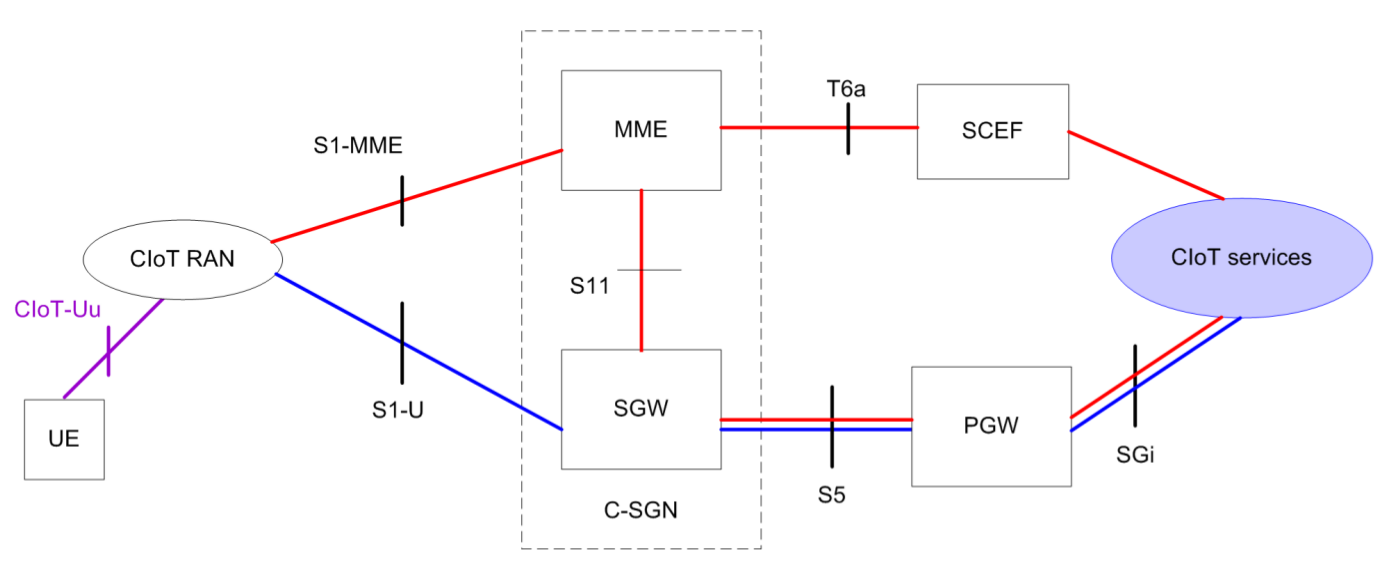
\includegraphics[width=\textwidth]{figures/NB-Network.png}
\definecolor{purple}{HTML}{7030A0}
\usetikzlibrary{arrows}
\definecolor{red}{HTML}{FF0000}
\definecolor{blue}{HTML}{00B0F0}

\resizebox{\textwidth}{!}{
\begin{tikzpicture}[scale=0.5]


\draw  (-14,5) rectangle (-10,3);
\node at (-12,4) {Device};
\draw  (-4,14) rectangle (2,-8);
\draw  (6,9) rectangle (10,7);
\draw  (6,1) rectangle (10,-1);
\node at (-1,-7) {\acrshort{CIoT} \acrshort{RAN}};
\node at (8,8) {\acrshort{MME}};
\node at (8,0) {\acrshort{SGW}};
 




\draw  (14,1) rectangle (18,-1);
\draw  (14,13) rectangle (18,11);
\draw  (25,6) ellipse (3 and 2);
\node at (16,12) {\acrshort{SCEF}};

\node at (16,0) {\acrshort{PGW}};
\node at (25,6) {\acrshort{CIoT} Services};

\draw  (-3,13) rectangle (1,11);
\draw  (-3,5) rectangle (1,3);
\draw  (-3,-3) rectangle (1,-5);
\node at (-1,12) {\acrshort{eNB}};
\node at (-1,4) {\acrshort{eNB}};
\node at (-1,-4) {\acrshort{eNB}};

\draw (6,18) -- (6,15); 
\draw (10,15) -- (10,18);
\draw  (8,18) ellipse (2 and 0.5);
\node at (8,15.4) {\acrshort{HSS}};
\draw (6,15) arc (-120:-60:4);

\draw (14,8.6) -- (14,5.6);
\draw (18,5.6) -- (18,8.6);
\draw  (16,8.6) ellipse (2 and 0.5);
\node at (16,6) {\acrshort{PCRF}};
\draw (14,5.6) arc (-120:-60:4);
\node (v27) at (16,5) {};


\node (v2) at (-7,4) {\acrshort{CIoT}-Uu};
\node (v1) at (-10,4) {};
\node (v3) at (-4,4) {};
\draw [draw=purple, arrows={triangle 45-},fill=purple] (v1) edge (v2);
\draw [draw=purple, arrows={-triangle 45},fill=purple] (v2) edge (v3);

\node (v5) at (-1,8) {X2};
\node (v8) at (-1,0) {X2};
\node (v4) at (-1,11) {};
\node (v6) at (-1,5) {};
\node (v7) at (-1,3) {};
\node (v9) at (-1,-3) {};
\draw [draw=red, arrows={triangle 45-},fill=red] (v4) edge (v5);
\draw [draw=red, arrows={-triangle 45},fill=red] (v5) edge (v6);
\draw [draw=red, arrows={triangle 45-},fill=red] (v7) edge (v8);
\draw [draw=red, arrows={-triangle 45},fill=red] (v8) edge (v9);
\node (v10) at (2,4) {};
\node (v14) at (6,0) {};
\node (v12) at (6,8) {};
\node (v18) at (8,7) {};
\node (v20) at (8,1) {};
\node (v17) at (8,9) {};
\node (v15) at (8,14.4) {};
\node (v21) at (10,8) {};
\node (v23) at (14,12) {};

\node (v24) at (10,0) {};
\node (v26) at (14,0) {};

\node (v33) at (18,0) {};
\node (v32) at (22,6) {};
\node (v30) at (18,12) {};
\node (v29) at (16,1) {};

\node (v11) at (4,6) {S1-\acrshort{MME}};
\node (v13) at (4,2) {S1-U};
\node (v19) at (8,4) {S11};
\node (v16) at (8,12) {S6a};
\node (v22) at (12,10) {T6a};
\node (v25) at (12,0) {S5};
\node (v28) at (16,3) {S7};
%\node (v31) at (20,9) {};
\node (v34) at (20,3) {SGi};

\draw [draw=red, arrows={triangle 45-},fill=red]  (v10) edge (v11);
\draw [draw=red, arrows={-triangle 45},fill=red]  (v11) edge (v12);
\draw [draw=blue, arrows={triangle 45-},fill=blue]  (v10) edge (v13);
\draw [draw=blue, arrows={-triangle 45},fill=blue]  (v13) edge (v14);


\draw [draw=red, arrows={triangle 45-},fill=red]   (v15) edge (v16);
\draw [draw=red, arrows={-triangle 45},fill=red]  (v16) edge (v17);
\draw [draw=red, arrows={triangle 45-},fill=red]  (v18) edge (v19);
\draw [draw=red, arrows={-triangle 45},fill=red]  (v19) edge (v20);
\draw [draw=red, arrows={triangle 45-},fill=red]  (v21) edge (v22);
\draw [draw=red, arrows={-triangle 45},fill=red]  (v22) edge (v23);
\draw [draw=purple, arrows={triangle 45-},fill=purple]  (v24) edge (v25);
\draw [draw=purple, arrows={-triangle 45},fill=purple]  (v25) edge (v26);
\draw [draw=red, arrows={triangle 45-},fill=red]  (v27) edge (v28);
\draw [draw=red, arrows={-triangle 45},fill=red]  (v28) edge (v29);
\draw [draw=red, arrows={triangle 45-triangle 45},fill=red]  (v30) edge (v32);
%\draw [draw=red, arrows={-triangle 45},fill=red]  (v31) edge (v32);
\draw [draw=purple, arrows={triangle 45-},fill=purple]  (v33) edge (v34);
\draw [draw=purple, arrows={-triangle 45},fill=purple]  (v34) edge (v32);
\end{tikzpicture}
}
\caption{Overview over the network blocks and interfaces between blocks in \gls{NB-IoT}. Blue lines are user plane \gls{CIoT} \gls{EPS} optimization, the red lines are control plane \gls{CIoT} \gls{EPS} optimization plane and the purple lines are both \citep{NB_slide}}
\label{fig:network_structure}
\end{figure}


\textbf{\gls{UE}}\\
The \gls{UE} is the smart meters or other products as mentioned, they do not need to transmit a lot of data and it is not critical that it arrives within a certain time frame. They do however require a long battery life time. The problem comes in terms of placement, because many of these devices might be placed in basement like environment which means an increased path loss. The system needs to be able to operate with a \gls{MCL} of 164 dB \citep{REL-13}. As in previous systems the \gls{USIM} is located on the \gls{UE} for authentication purpose \citep[ch. 3]{book_LTE_for_UMTS}.

\textbf{\gls{CIoT} \gls{RAN}}\\
The \gls{CIoT} \gls{RAN} is the base stations, the most typically used is the \gls{eNB} base station. All radio communication terminates at this node. Any \gls{UE} that wish to use an external service, interfaces with the \gls{eNB} \citep{book_LTE_for_UMTS}. The \gls{eNB} interfaces with both the \gls{MME} and the \gls{SGW}. On the control plane (connection to the \gls{MME}) the \gls{eNB} is in charge of \gls{RRM}, i.e. allocating radio resources in the user plane to the individual \gls{UE} based on \gls{QoS} measures. 

\textbf{\gls{MME}}\\
The \gls{MME} takes care of mobility issues, it also keep track of where in the network different \gls{UE}s are connected \citepalias{3GPP_MME_spec}. Another very important function of the \gls{MME} is to handle authentication of \gls{UE}s and setting up security for the data bearers. The \gls{MME} might be connected to multiple \gls{UE}s, however a \gls{UE} may only be connected to a single \gls{MME} \citep[ch. 3]{book_LTE_for_UMTS}. In \gls{NB-IoT} handovers are omitted and the only way to change cell is by releasing the existing connection \citep{REL-13}. The \gls{MME} also handles paging procedures \citep{NB-IoT_Book}.

\textbf{\gls{HSS}}\\
The \gls{HSS} stores the identity of the users, which the \gls{MME} uses for authentication purposes. It records the location of the \gls{UE} in level of visited network control nodes  such as \gls{MME}, it also keep track of which networks the user is allowed to roam to \citep[ch. 3]{book_LTE_for_UMTS}.

\textbf{\gls{SCEF}}\\
The \gls{SCEF} is a multi functional unit, task it handles include: device trigger delivery, sponsored data, \gls{UE} reachability, \gls{3GPP} network issues, \gls{QoS} for a \gls{UE} session etc. Many of these functionalities are meant for normal \gls{LTE} use. Uses meant for \gls{NB-IoT} include \gls{UE} reachability which enables the application layer to be informed when a \gls{UE} reconnects to the network i.e. after an \gls{eDRX} or after \gls{PSM}. Another functionality it handles is \gls{NIDD}, which enables \gls{UE}s with small data volumes to send it data with less overhead and thereby have a longer battery life time \citepalias{3GPP_SCEF_primer}.

\textbf{\gls{SGW}}\\
The \gls{SGW} is primarily a routing unit. It interfaces with the \gls{eNB}, the \gls{MME} and the \gls{PGW}. When the \gls{UE} transmit data it is send to the \gls{eNB} and then routed via the \gls{SGW} to the \gls{PGW} before reaching the providers. The \gls{SGW} typically serve a particular geographic area with several \gls{eNB}s, likewise could the \gls{MME} also serve a particular geographic area. In \gls{LTE} this was the last node in the network that could change during a connected state meaning that all \gls{SGW}s needs to be connected to all \gls{PGW}s \citep[ch. 3]{book_LTE_for_UMTS}. This is however not equally important in \gls{NB-IoT} as no handovers are expected \citep{REL-13}. During connected state the \gls{SGW} works as a relay, however in idle mode the resources are released in the \gls{eNB} and the data path terminates at the \gls{SGW} it then stores the data from the \gls{PGW} and request the \gls{MME} to initiate paging of the \gls{UE} \citep[ch. 3]{book_LTE_for_UMTS}.

\textbf{\gls{PGW}}\\
The \gls{PGW} is the edge of the \gls{EPS}. It function as the point of attachment for the \gls{UE}s \gls{IP} traffic. The \gls{IP}-address of the \gls{UE} is allocated during the connection procedure when the \gls{UE} request a \gls{PDN} connection and during any subsequent \gls{PDN} connection request. It is the \gls{PGW} that performs the \gls{DHCP} functionality \citep[ch. 3]{book_LTE_for_UMTS}. The \gls{PGW} handle interfaces to external CIoT services on a higher level.

\textbf{\gls{PCRF}}\\
The \gls{PCRF} is a server that makes decision on how to handle services provided for the \gls{UE} in terms of \gls{QoS}. It informs the \gls{PGW} and if applicable the \gls{SGW} about appropriate bearer policy can be set up. A default bearer is set up during connection request and either the \gls{UE} or the service domain can request additional bearers which is handled by the \gls{PCRF} \citep[ch. 3]{book_LTE_for_UMTS}.

\textbf{\gls{CIoT} services}\\
The \gls{CIoT} services are typically storage functionalities, but could be control algorithms or other services needed for specific products. 

%connections across the network

\section{Protocol Layers}

The following section is focused on the communication protocol in the \gls{CIoT}-Uu interface. It consist of the following six layers:
\begin{itemize}
	\item \gls{NAS} layer
	\item \gls{RRC} layer
	\item \gls{PDCP} layer
	\item \gls{RLC} layer
	\item \gls{MAC} layer
	\item \gls{PHY} layer
\end{itemize}

The purpose and functionalities of these layers are explained in the following.

\subsection{NAS}
The \gls{NAS} layer is the top layer in the control plane. It signals directly between the device and the \gls{MME} \citep[ch. 3]{book_LTE_for_UMTS}. There are two protocols in the \gls{NAS} layer, the \gls{EMM} and the \gls{ESM}. The \gls{EMM} handles re-activation from idle mode: the device initiated case is called service request, the network initiated case is called paging. The \gls{EMM} protocol is used for handling attachment and detachment from the system when the device is in idle mode. In connected mode lower layer protocols handles this instead \citep[ch. 3]{book_LTE_for_UMTS}. In the NB-IoT protocol, a functionality has been implemented, to transmit data directly through the NAS layer \citep{REL-13}. 

\subsection{RRC} \label{sec:RRC}
The \gls{RRC} layer of the protocol is a strictly control plane layer. The functionalities provided by the \gls{RRC} are \citep[ch. 6.6]{book_LTE_for_UMTS}:

\begin{itemize}
	\item Broadcast of system information
	\item Paging
	\item Establishment, maintenance and release of an \gls{RRC} connection between device and the \gls{eNB}
	\item Security functions, including key management
	\item Establishment, maintenance and release of point to point radio bearers
	\item Device measurement reporting and control of the reporting
	%\item Handover
	\item Device cell selection and reselections 
%	\item Context transfer between \gls{eNB}s
	\item Device capability transfer
	\item Generic protocol error handling
	\item Support of self-configuration and self-optimization
\end{itemize}

One of the biggest changes from \gls{LTE} to \gls{NB-IoT} is the focus on reducing power consumption. Therefore a new state has been introduced compared to the \gls{LTE} system, which can be seen on \autoref{fig:UE-states}.

\tikzsetnextfilename{state-diagram}
\begin{figure}[H]
\centering
\usetikzlibrary{arrows}
%\usetikzlibrary{shapes.multipart}
\renewcommand{\arraystretch}{0.8}
\resizebox{\textwidth}{!}{
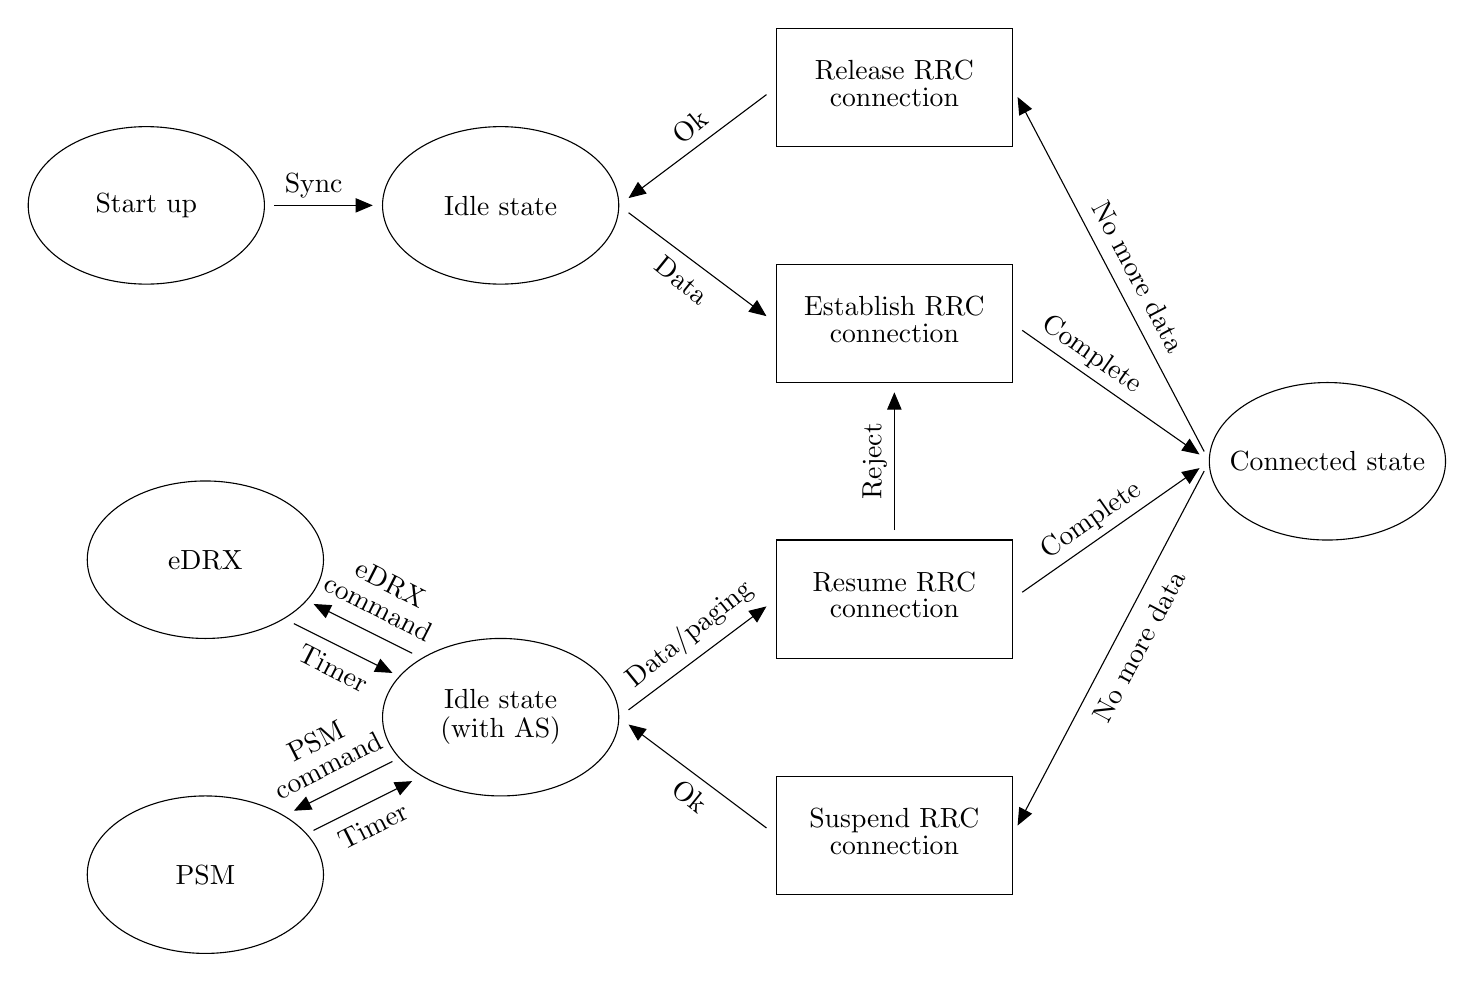
\begin{tikzpicture}[scale=0.5]

\draw  (-26,28) ellipse (3 and 2);
\node at (-26,28) {Start up};

\draw  (-17,28) ellipse (3 and 2);
\node at (-17,28) {Idle state};

\draw  (-24.5,11) ellipse (3 and 2);
%\node at (-17,15) {\acrshort{PSM}};
\node at (-24.5,11) {PSM};

\draw  (-10,19.5) rectangle (-4,16.5);
\node at (-7,18) {\begin{tabular}{c} Resume RRC \\ connection \end{tabular}};

\draw  (-10,26.5) rectangle (-4,23.5);
\node at (-7,25) {\begin{tabular}{c} Establish RRC \\ connection\end{tabular}};

\draw  (-10,13.5) rectangle (-4,10.5);
\node at (-7,12) {\begin{tabular}{c} Suspend RRC \\ connection\end{tabular}};

\draw  (-10,32.5) rectangle (-4,29.5);
\node at (-7,31) {\begin{tabular}{c} Release RRC \\ connection\end{tabular}};

\draw  (4,21.5) ellipse (3 and 2);
\node at (4,21.5) {Connected state};

\draw  (-17,15) ellipse (3 and 2);
\node at (-17,15) {\begin{tabular}{c} Idle state \\ (with AS)\end{tabular}};
\node (v22) at (-20,15) {};
\node (v23) at (-14,15) {};

\draw  (-24.5,19) ellipse (3 and 2);
\node at (-24.5,19) {eDRX};
\node (v25) at (-19,16.5) {};
\node (v26) at (-22,18) {};
\node (v27) at (-22.5,17.5) {};
\node (v28) at (-19.5,16) {};
\node[rotate=27] at (-21.5,14) {\begin{tabular}{c} PSM\\ command\end{tabular}};
\node[rotate=27] at (-20.25,12.25) {Timer};




\node (v1) at (-23,28) {};
\node (v2) at (-20,28) {};
\node (v3) at (-14,28) {};
\node (v4) at (-10,25) {};
\node (v5) at (-4,25) {};
\node (v6) at (1,21.5) {};
\node (v7) at (-4,12) {};
\node (v8) at (-4,31) {};
\node (v9) at (-4,18) {};
\node (v10) at (-10,18) {};
\node (v11) at (-10,12) {};
\node (v12) at (-10,31) {};
\node (v13) at (-7,19.5) {};
\node (v14) at (-7,23.5) {};
\node (v15) at (-19.5,14) {};
\node (v16) at (-22.5,12.5) {};
\node (v17) at (-22,12) {};
\node (v18) at (-19,13.5) {};



\draw [arrows={- triangle 45}] (v1) edge (v2);
\draw [arrows={- triangle 45}] (v23) edge (v10);
\draw [arrows={- triangle 45}] (v3) edge (v4);
%\draw [arrows={triangle 45-}]  (v4) edge ($(midpoint)+(0,0)$);

\draw [arrows={- triangle 45}] (v11) edge (v23);
\draw [arrows={- triangle 45}] (v12) edge (v3);
\draw [arrows={- triangle 45}] (v13) edge (v14);
\draw [arrows={- triangle 45}] (v9) edge (v6);
\draw [arrows={- triangle 45}] (v5) edge (v6);
\draw [arrows={- triangle 45}] (v6) edge (v7);
\draw [arrows={- triangle 45}] (v6) edge (v8);
\draw [arrows={- triangle 45}] (v15) edge (v16);
\draw [arrows={- triangle 45}]  (v17) edge (v18);
\draw [arrows={- triangle 45}] (v25) edge (v26);
\draw [arrows={- triangle 45}]  (v27) edge (v28);


\node at (-21.75,28.5) {Sync};
\node[rotate=-27] at (-20,18) {\begin{tabular}{c} eDRX \\ command\end{tabular}};
\node[rotate=-27] at (-21.25,16.25) {Timer};
\node[rotate=39] at (-12.2,30) {Ok};
\node[rotate=39] at (-12.2,17.1) {Data/paging};
\node[rotate=-39] at (-12.2,13) {Ok};
\node[rotate=-39] at (-12.4,26.1) {Data};
\node[rotate=-35] at (-2,24.2) {Complete};
\node[rotate=35] at (-2,20) {Complete};
\node[rotate=62] at (-0.8,16.8) {No more data};
\node[rotate=-62] at (-0.8,26.2) {No more data};
\node[rotate=90] at (-7.5,21.5) {Reject};


\end{tikzpicture}
}
\caption{State diagram with transition options for a device.}
\label{fig:UE-states}
\end{figure}


With this new structure comes a greater focus on \gls{RRC} connection resume, which is very advantageous with regards to power consumption, as it allows the device to suspend its connection and save its \gls{AS}, when going into idle mode.

This enables the device to request a connection resume, where it uses its previous \gls{AS} to reduces the overhead considerably. This can also be seen from \autoref{tab:signaling_comparison} where a comparison between the different procedures is shown. 

\begin{table}[H]
\centering
\resizebox{\textwidth}{!}{
\begin{tabular}{|p{2.5cm}|p{4cm}|p{4cm}|p{4cm}|} \hline
\rowcolor{gray!50}\textbf{Direction} & \raggedright\arraybackslash\textbf{Legacy Service Request Procedure}	& \raggedright\arraybackslash\textbf{\gls{RRC} Connection Resume} & \textbf{Control Plane Data Transfer}  \\\hline
UL	& \multicolumn{3}{c|}{Preamble} \\\hline
\rowcolor{gray!10}DL	& \multicolumn{3}{c|}{\gls{RAR}} \\\hline
UL	& \raggedright\arraybackslash \gls{RRC} Connection Request						& \raggedright\arraybackslash \gls{RRC} Connection Resume Request	& \raggedright\arraybackslash \gls{RRC} Connection Request \\\hline
\rowcolor{gray!10}DL	& \raggedright\arraybackslash \gls{RRC} Connection Setup						& \raggedright\arraybackslash \gls{RRC} Connection Resume 			& \raggedright\arraybackslash \gls{RRC} Connection Setup   \\\hline
UL	& \raggedright\arraybackslash \gls{RRC} Connection Request Complete 			& \raggedright\arraybackslash \gls{RRC} Connection Resume Complete & \raggedright\arraybackslash \gls{RRC} Connection Complete  \\\hline
\rowcolor{gray!10}DL	& \raggedright\arraybackslash Security Mode Command 							& - & -  \\\hline
UL	& \raggedright\arraybackslash Security Mode Complete 							& - & -  \\\hline
\rowcolor{gray!10}DL	& \raggedright\arraybackslash \gls{RRC} Connection Reconfiguration 			& - & -  \\\hline
UL	& \raggedright\arraybackslash \gls{RRC} Connection Reconfiguration Complete 	& - & -  \\\hline
\raggedright\arraybackslash \textbf{Total number of messages} 					& \textbf{9} & \textbf{5} & \textbf{5} \\\hline
\end{tabular}
}
\caption{Signaling comparison between different methods \citep{REL-13}.}
\label{tab:signaling_comparison}
\end{table}

\textbf{\Gls{SRB}}\\
The \gls{RRC} sets up three different \gls{SRB}s, which are used to carry \gls{RRC} and \gls{NAS} messages. \gls{SRB}0 is used for \gls{CCCH} during \gls{RRC} connection setup or during link failure. Messages carried here include \gls{RRC} connection request, \gls{RRC} connection setup, \gls{RRC} connection reject, \gls{RRC} connection reestablishment request, \gls{RRC} connection reestablishment and \gls{RRC} connection reestablishment reject. \gls{SRB}1 is used when a \gls{RRC} connection is established. It is used to transfer both \gls{RRC} messages, using \gls{DCCH}, and \gls{NAS} messages until security is established. Once security is established, the \gls{NAS} messages is carried on \gls{SRB}2, which has a lower priority. \citep[ch. 6.6]{book_LTE_for_UMTS} 


\textbf{\gls{SIB}s}\\
Before the device attempts to access the system, it needs a lot of information about the system, which is carried in the \gls{SIB}s. For \gls{NB-IoT} there are eight different \gls{SIB}s messages. A list of the information carried in the different \gls{SIB}s can be seen in \autoref{tab:NB-SIB}. The \gls{RRC} takes care of updating these messages and paging the devices if changes occurs.

\begin{table}[H]
\centering
\begin{tabular}{|p{3cm}|p{8cm}|p{3cm}|}\hline
\textbf{Name}		& \textbf{Information}																	& \textbf{Update rate}	\\\hline
\raggedright\arraybackslash\gls{MIB-NB}		& Essential information required to receive further system information 					& 640 ms				\\\hline
\raggedright\arraybackslash\gls{NB-SIB}1		& Cell access and selection and the other SIBs scheduling 										& 40.96 s 				\\\hline
\gls{NB-SIB}2		& Radio resource configuration information 												& NA 					\\\hline
\gls{NB-SIB}3		& Cell re-selection information for intra-frequency, inter-frequency 					& NA 					\\\hline
\gls{NB-SIB}4		& Neighboring cell related information relevant for intra-frequency cell re-selection 	& NA 					\\\hline
\gls{NB-SIB}5		& Neighboring cell related information relevant for inter-frequency cell re-selection 	& NA 					\\\hline
\gls{NB-SIB}14		& Access barring parameters 															& Fast 					\\\hline
\gls{NB-SIB}16		& Information related to GPS time and Coordinated Universal Time (UTC) 					& Fast 					\\\hline
\end{tabular}
\caption{List of different \gls{SIB} messages and the information carried within \citep{whitepaper,REL-13}.}
\label{tab:NB-SIB}
\end{table}

\textbf{Paging} \\
Paging serves two main functions: the first is to notify a device in \gls{RRC} idle state to set up a \gls{RRC} connection to handle incoming data and the second is to inform the devices, both in \gls{RRC} idle and \gls{RRC} connected state, that the system information has changed. \citep[ch. 7]{NB-IoT_Book}

\textbf{Establishment, Maintenance and Release of \gls{RRC} Connection} \\
When an \gls{RRC} connection setup is requested, the \gls{eNB} has the option to reject it with a wait timer, if the network is overloaded. The \gls{RRC} can set the access barring parameter appropriately depending on the traffic load. In the \gls{RRC} connection request message, the device can trasmit its \gls{S-TMSI} if it possess a valid version, else it will transmit a 40 bit random value. Five different establishment causes has been defined: emergency, high-priority access, mobility-terminated access, mobile-originated signaling and mobile-originated data. In \gls{NB-SIB}1 there exists at most six different \gls{PLMN} identities, where the device selects one and reports it in the  \gls{RRC} connection setup complete message, along with any \gls{MME} the device might already be registered to. The \gls{eNB} then finds the \gls{MME} and starts the S1 connection setup. When a connection setup is successful the device moves to the \gls{RRC} connected state. \citep[ch. 6.6]{book_LTE_for_UMTS}

%\todo{should we put detailed connection options in here, should we go in detail with further RRC functions and what about radio bearers}

%\textbf{\gls{UE} Measurement Reporting and Control of the Reporting} \\


%%% pic for rrc connection resume
%\begin{figure}[H]
%\centering
%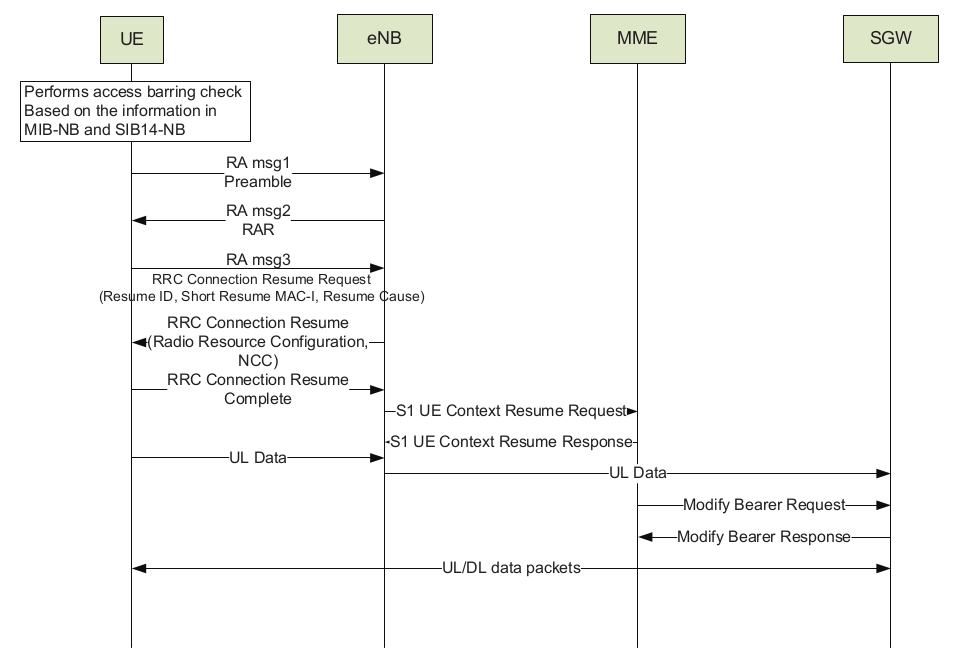
\includegraphics[width=\textwidth]{figures/RRC_resume.png}
%\caption{Signaling procedure for a \gls{RRC} resume request}
%\label{fig:RRC_resume}
%\end{figure}

\subsection{PDCP}
The \gls{PDCP} layer is just below the \gls{RRC}, where it handles both control functions as well as device data. The key function of the \gls{PDCP} include \citep[ch. 6.5]{book_LTE_for_UMTS}:
\begin{itemize}
	\item Header compression and decompression of \gls{IP} packets. This is an important function especially for small data packets, as the overhead could become quite significant
	\item Ciphering and deciphering of both user plane and most of control plane data
	\item Integrity protection and verification to ensure control data comes from the correct source
\end{itemize}

The \gls{PDCP} gets \gls{PDCP} \gls{SDU}s from the \gls{RRC} and \gls{NAS} layer. 

\tikzsetnextfilename{PDCP_data_flow}
\begin{figure}[H]
\centering
\resizebox{0.8\textwidth}{!}{
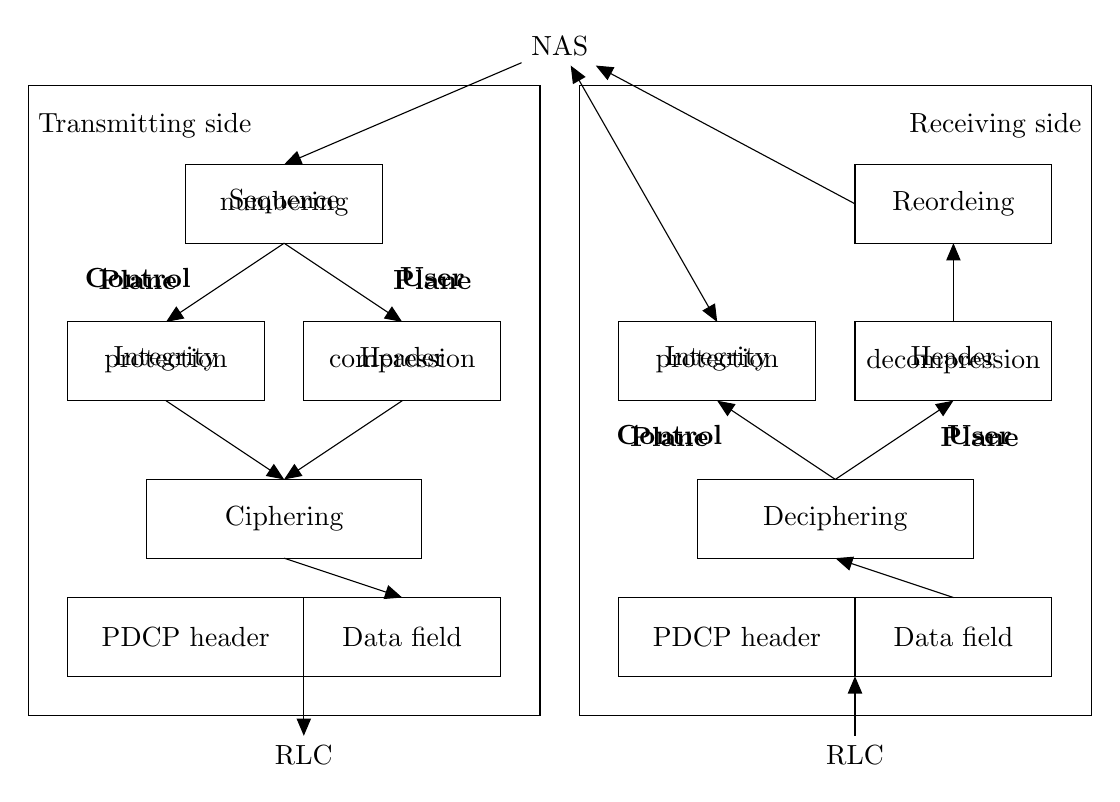
\begin{tikzpicture}[scale=.5]


\node (v2) at (-0.5,8) {NAS};
\draw  (-1,7) rectangle (-14,-9);
\draw  (0,7) rectangle (13,-9);
\node[anchor=west] at (-14,6) {Transmitting side};
\node[anchor=east] at (13,6) {Receiving side};

\draw  (-10,5) rectangle (-5,3);
\node at (-7.5,4) {\begin{tabular}{c} Sequence \\[-0.9em] numbering \end{tabular}};
\draw  (-13,1) rectangle (-8,-1);
\node at (-10.5,0) {\begin{tabular}{c} Integrity \\[-0.9em] protection \end{tabular}};
\draw  (-7,1) rectangle (-2,-1);
\node at (-4.5,0) {\begin{tabular}{c} Header \\[-0.9em] compression \end{tabular}};
\draw  (-11,-3) rectangle (-4,-5);
\node at (-7.5,-4) {Ciphering};
\draw  (-13,-6) rectangle (-7,-8) node (v1) {};
\draw  (v1) rectangle (-2,-6);
\node at (-10,-7) {PDCP header};
\node at (-4.5,-7) {Data field};
\node (v12) at (-7,-10) {RLC};

\node (v3) at (-7.5,5) {};
\node (v4) at (-7.5,3) {};
\node (v5) at (-10.5,1) {};
\node (v6) at (-4.5,1) {};
\node (v9) at (-4.5,-1) {};
\node (v7) at (-10.5,-1) {};
\node (v8) at (-7.5,-3) {};
\node (v10) at (-7,-5) {};
\node (v11) at (-4.5,-6) {};
\draw  [- triangle 45] (v2) -- (-7.5,5);
\draw  [- triangle 45] (-7.5,3) -- (-10.5,1);
\draw  [- triangle 45] (-7.5,3) -- (-4.5,1);
\draw  [- triangle 45] (-10.5,-1) -- (-7.5,-3);
\draw  [- triangle 45] (-4.5,-1) -- (-7.5,-3);
\draw  [- triangle 45] (-7.5,-5) -- (-4.5,-6);
\draw  [- triangle 45] (-7,-8) -- (v12);
\node[anchor=east] at (-9.2,2) {\begin{tabular}{c} \textbf{Control} \\[-0.9em] \textbf{Plane} \end{tabular}};
\node[anchor=west] at (-5.4,2) {\begin{tabular}{c} \textbf{User} \\[-0.9em] \textbf{Plane} \end{tabular}};

\draw  (12,5) rectangle (7,3);
\node at (9.5,4) {Reordeing};
\draw  (6,1) rectangle (1,-1);
\node at (3.5,0) {\begin{tabular}{c} Integrity \\[-0.9em] protection \end{tabular}};
\draw  (12,1) rectangle (7,-1);
\node at (9.5,0) {\begin{tabular}{c} Header \\[-0.9em] decompression \end{tabular}};
\draw  (10,-3) rectangle (3,-5);
\node at (6.5,-4) {Deciphering};
\draw  (12,-6) rectangle (7,-8) node (v1) {};
\draw  (v1) rectangle (1,-6);
\node at (4,-7) {PDCP header};
\node at (9.5,-7) {Data field};

\node (v3) at (-7.5,5) {};
\node (v4) at (-7.5,3) {};
\node (v5) at (3.5,1) {};
\node (v6) at (9.5,1) {};
\node (v9) at (9.5,-1) {};
\node (v7) at (3.5,-1) {};
\node (v8) at (6.5,-3) {};
\node (v10) at (6,-5) {};
\node (v11) at (9.5,-6) {};
\node (v14) at (9.5,3) {};
\node (v15) at (7,4) {};
\node (v13) at (7,-10) {RLC};

\draw [- triangle 45] (v13) -- (7,-8);
\draw [- triangle 45] (9.5,-6) -- (6.5,-5);
\draw [- triangle 45] (6.5,-3) -- (3.5,-1);
\draw [- triangle 45] (6.5,-3) -- (9.5,-1);
\draw [- triangle 45] (9.5,1) -- (9.5,3);
\draw [- triangle 45] (7,4) -- (v2);
\draw [arrows={triangle 45 - triangle 45}] (3.5,1) -- (v2);
\node[anchor=east] at (4.3,-2) {\begin{tabular}{c} \textbf{Control} \\[-0.9em] \textbf{Plane} \end{tabular}};
\node[anchor=west] at (8.5,-2) {\begin{tabular}{c} \textbf{User} \\[-0.9em] \textbf{Plane} \end{tabular}};

\end{tikzpicture}}
\caption{\gls{PDCP} layer operation with associated \gls{PDCP} \gls{SDU} \citep[fig. 6.12]{book_LTE_for_UMTS}.}
\label{fig:PDCP_operation}
\end{figure}

As can be seen on \autoref{fig:PDCP_operation}, before forwarding the data to the \gls{RLC} layer, it is first numbered and then either integrity protection or header compression is applied, depending on whether or not it is control plane data or user plane data. It is then ciphered and forwarded. When the \gls{PDCP} receive data from the \gls{RLC} layer, it is first deciphered and again depending on whether it is control or user plane data, is it integrity protected or header decompressed and reordered, before forwarding it to the \gls{NAS}. \citep[ch. 6.5]{book_LTE_for_UMTS}  

%The \gls{PDCP} layer also handles alot during handovers, however as handovers is out of the scope for \gls{NB-IoT} these functionalities are obsolete. 

\subsection{RLC}

The \gls{RLC} layer has three basic functionalities \cite[ch. 6.4]{book_LTE_for_UMTS}:

\begin{itemize}
	\item To transfer \gls{PDU}s from higher layers i.e. \gls{RRC}, \gls{NAS} or \gls{PDCP}
	\item Depending on the \gls{RLC} mode used, error correction with \gls{ARQ}, concatenation/segmentation, in-sequence delivery and duplicate detection may occur
	\item Protocol error handling to detect and recover from protocol error states caused by e.g. signaling errors
\end{itemize}

\captionsetup{belowskip=0em}
\begin{minipage}[H]{0.48\textwidth}
\tikzsetnextfilename{RLC_UM-SAP}
\begin{figure}[H]
\centering
\resizebox{\textwidth}{!}{
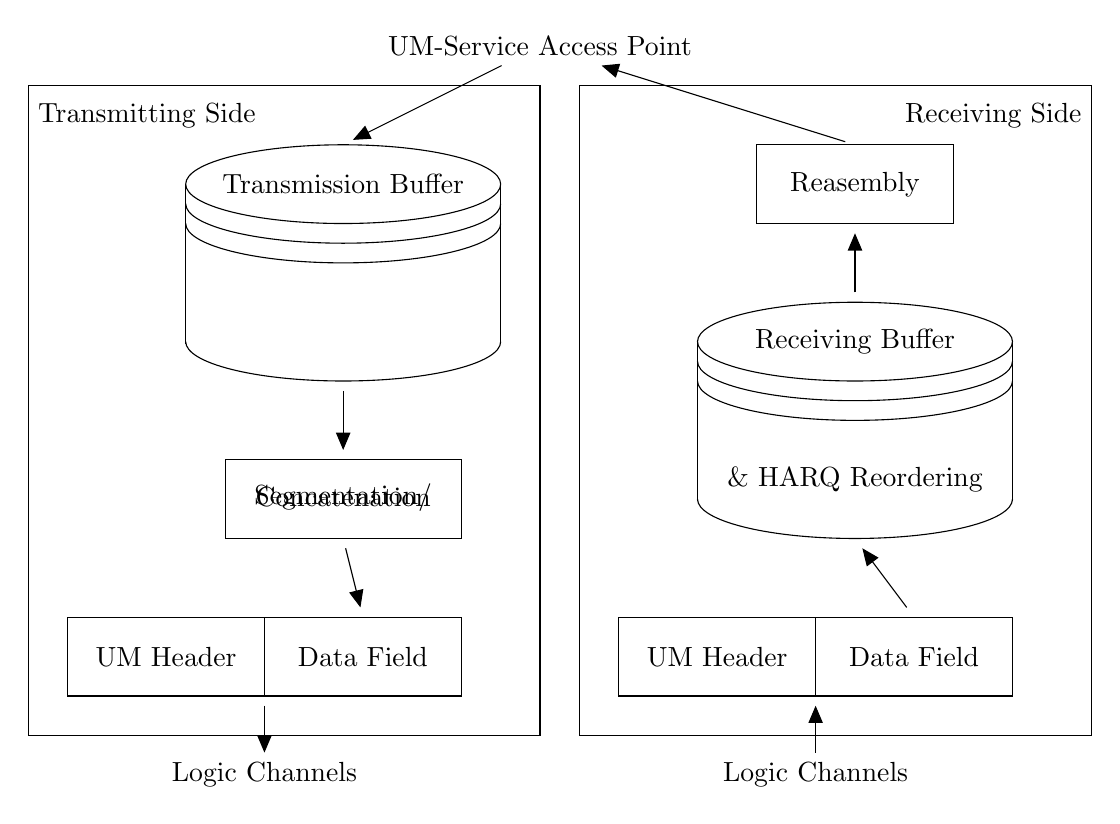
\begin{tikzpicture}[scale=.5]

\draw  (-1,8.5) rectangle (-14,-8);
\draw  (0,8.5) rectangle (13,-8);

\node (v1) at (-6,6) {Transmission Buffer};
\draw  (v1) ellipse (4 and 1);
\draw (-10,5.5) arc (180:360:4 and 1);
\draw (-10,5) arc (180:360:4 and 1);
\draw (-10,2) arc (180:360:4 and 1);
\node (v2) at (-10,6) {};
\node (v4) at (-2,6) {};
\node (v3) at (-10,1.7) {};
\node (v5) at (-2,1.7) {};
\draw  (v2) ++(0,0) edge (v3);
\draw  (v4)  ++(0,0) edge (v5);

\draw  (-9,-1) rectangle (-3,-3);
\node at (-6,-2) {\begin{tabular}{c} Segmentation/ \\[-0.9em] Concatenation\end{tabular}};
\draw  (-13,-5) rectangle (-8,-7) node (v6) {};
\draw  (v6) rectangle (-3,-5);
\node at (-10.5,-6) {UM Header};
\node at (-5.5,-6) {Data Field};



\node (v10) at (7,2) {Receiving Buffer};
\draw  (v10) ellipse (4 and 1);
\draw (3,1.5) arc (180:360:4 and 1);
\draw (3,1) arc (180:360:4 and 1);
\draw (3,-2) arc (180:360:4 and 1);
\node (v20) at (3,2) {};
\node (v40) at (11,2) {};
\node (v30) at (3,-2.3) {};
\node (v50) at (11,-2.3) {};
\draw  (v20) ++(0,0) edge (v30);
\draw  (v40)  ++(0,0) edge (v50);


\draw  (4.5,7) rectangle (9.5,5);
\draw  (1,-5) rectangle (6,-7) node (v7) {};
\draw  (v7) rectangle (11,-5);
\node at (7,6) {Reasembly};
\node at (7,-1.5) {\& HARQ Reordering};
\node at (3.5,-6) {UM Header};
\node at (8.5,-6) {Data Field};

\node (v15) at (-8,-9) {Logic Channels};
\node (v16) at (6,-9) {Logic Channels};
\node (v14) at (-5.5,-5) {};
\node (v13) at (-6,-3) {};
\node (v11) at (-6,1) {};
\node (v9) at (-6,7) {};
\node (v8) at (-1,9.5) {UM-Service Access Point};
\node (v22) at (7,7) {};
\node (v21) at (7,5) {};
\node (v19) at (7,3) {};
\node (v18) at (7,-3) {};
\node (v17) at (8.5,-5) {};
\node (v12) at (-6,-1) {};

\draw [arrows={ - triangle 45}] (v8) edge (v9);
\draw [arrows={ - triangle 45}] (v11) edge (v12);
\draw [arrows={ - triangle 45}] (v13) edge (v14);
\draw [arrows={ - triangle 45}] (v6) edge (v15);
\draw [arrows={ - triangle 45}] (v16) edge (v7);
\draw [arrows={ - triangle 45}] (v17) edge (v18);
\draw [arrows={ - triangle 45}] (v19) edge (v21);
\draw [arrows={ - triangle 45}] (v22) edge (v8);
\node [anchor=west] at (-14,7.75) {Transmitting Side};
\node [anchor=east] at (13,7.75) {Receiving Side};
\end{tikzpicture}}
\caption{\gls{RLC} \gls{UM} operation \citep[ch. 6.4]{book_LTE_for_UMTS}.}
\label{fig:RLC_AM/UM_operation2}
\end{figure}
\end{minipage}
\begin{minipage}[H]{0.48\textwidth}
\begin{figure}[H]
\tikzsetnextfilename{RLC_AM-SAP}
\centering
\resizebox{\textwidth}{!}{
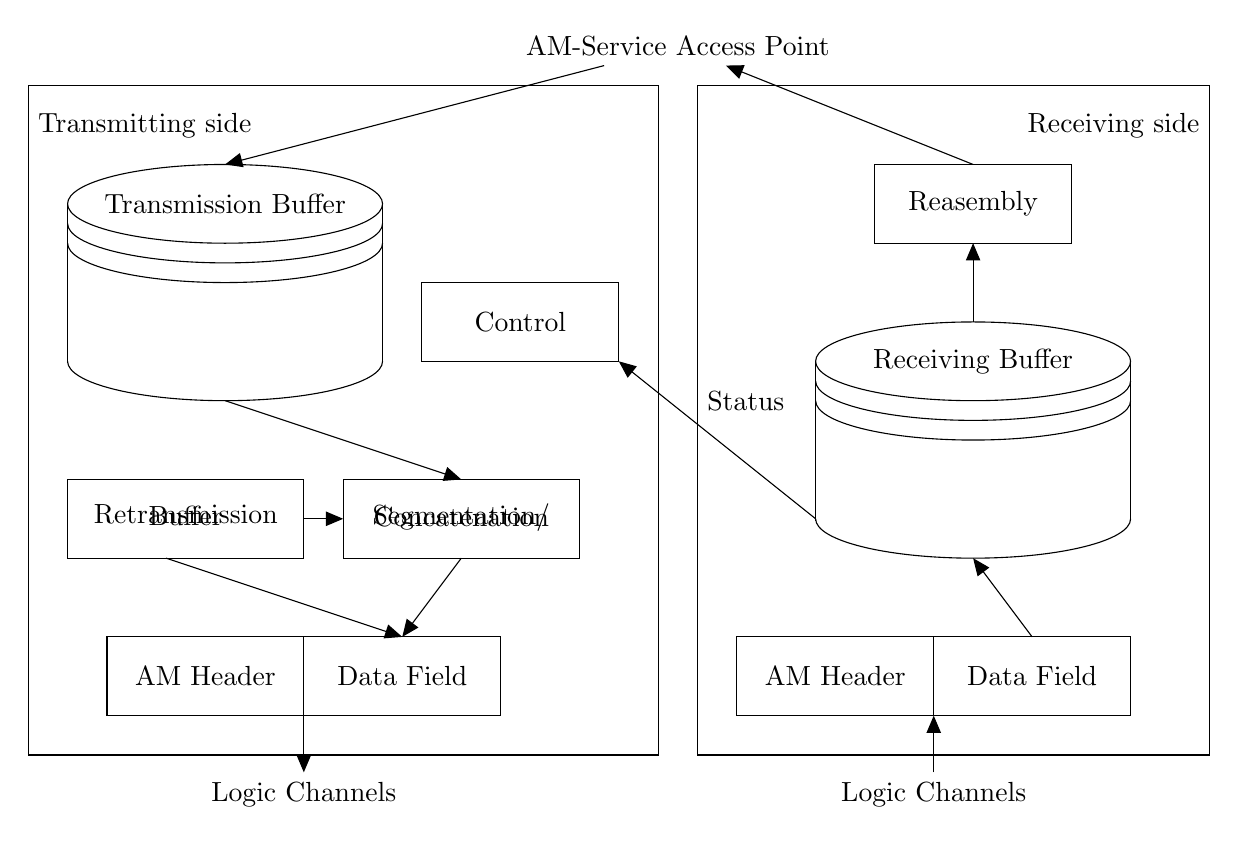
\begin{tikzpicture}[scale=.5]

\draw  (-1,9) rectangle (-17,-8);
\draw  (0,9) rectangle (13,-8);

\node (v1) at (-12,6) {Transmission Buffer};
\draw  (v1) ellipse (4 and 1);
\draw (-16,5.5) arc (180:360:4 and 1);
\draw (-16,5) arc (180:360:4 and 1);
\draw (-16,2) arc (180:360:4 and 1);
\node (v2) at (-16,6) {};
\node (v4) at (-8,6) {};
\node (v3) at (-16,1.7) {};
\node (v5) at (-8,1.7) {};
\draw  (v2) ++(0,0) edge (v3);
\draw  (v4)  ++(0,0) edge (v5);

\draw  (-9,-1) rectangle (-3,-3);
\node at (-6,-2) {\begin{tabular}{c} Segmentation/ \\[-0.9em] Concatenation\end{tabular}};
\draw  (-15,-5) rectangle (-10,-7) node (v6) {};
\draw  (v6) rectangle (-5,-5);
\node at (-12.5,-6) {AM Header};
\node at (-7.5,-6) {Data Field};



\node (v10) at (7,2) {Receiving Buffer};
\draw  (v10) ellipse (4 and 1);
\draw (3,1.5) arc (180:360:4 and 1);
\draw (3,1) arc (180:360:4 and 1);
\draw (3,-2) node (v23) {} arc (180:360:4 and 1);
\node (v20) at (3,2) {};
\node (v40) at (11,2) {};
\node (v30) at (3,-2.3) {};
\node (v50) at (11,-2.3) {};
\draw  (v20) ++(0,0) edge (v30);
\draw  (v40)  ++(0,0) edge (v50);


\draw  (4.5,7) rectangle (9.5,5);
\draw  (1,-5) rectangle (6,-7) node (v7) {};
\draw  (v7) rectangle (11,-5);
\node at (7,6) {Reasembly};
\node at (7,-1.5) {};
\node at (3.5,-6) {AM Header};
\node at (8.5,-6) {Data Field};

\node (v15) at (-10,-9) {Logic Channels};
\node (v16) at (6,-9) {Logic Channels};
\node (v14) at (-7.5,-5) {};
\node (v13) at (-6,-3) {};
\node (v11) at (-12,1) {};
\node (v9) at (-12,7) {};
\node (v8) at (-0.5,10) {AM-Service Access Point};
\node (v22) at (7,7) {};
\node (v21) at (7,5) {};
\node (v19) at (7,3) {};
\node (v18) at (7,-3) {};
\node (v17) at (8.5,-5) {};
\node (v12) at (-6,-1) {};

\draw [arrows={ - triangle 45}] (v8) -- (-12,7);
\draw [arrows={ - triangle 45}] (-12,1) -- (-6,-1);
\draw [arrows={ - triangle 45}] (-6,-3) -- (-7.5,-5);
\draw [arrows={ - triangle 45}] (-10,-7) -- (v15);
\draw [arrows={ - triangle 45}] (v16) -- (6,-7);
\draw [arrows={ - triangle 45}] (8.5,-5) -- (7,-3);
\draw [arrows={ - triangle 45}] (7,3) -- (7,5);
\draw [arrows={ - triangle 45}] (7,7) -- (v8);
\node [anchor=west] at (-17,8) {Transmitting side};
\node [anchor=east] at (13,8) {Receiving side};
\draw  (-10,-1) rectangle (-16,-3);
\node at (-13,-2) {\begin{tabular}{c} Retransmission \\[-0.9em] Buffer\end{tabular}};
\draw  (-7,4) rectangle (-2,2) node (v24) {};
\node at (-4.5,3) {Control};
\draw [arrows={ - triangle 45}] (3,-2) -- (-2,2);
\node [anchor=west] at (0,1) {Status};
\node (v25) at (-10.2,-2) {};
\node (v26) at (-8.8,-2) {};
\node (v27) at (-13.5,-3) {};
\draw [arrows={ - triangle 45}] (-10,-2) -- (-9,-2);
\draw [arrows={ - triangle 45}] (-13.5,-3) -- (-7.5,-5);
\end{tikzpicture}}
\caption{\gls{RLC} \gls{AM} operation \citep[ch. 6.4]{book_LTE_for_UMTS}.}
\label{fig:RLC_AM/UM_operation}
\end{figure}
\end{minipage}
\captionsetup{belowskip=-1.5em}


The modes mentioned before include \gls{TM}, \gls{UM} and \gls{AM} \citep[ch. 6.4]{book_LTE_for_UMTS}, with the differences shown on \autoref{fig:RLC_AM/UM_operation} and \autoref{fig:RLC_AM/UM_operation2}, with the exception of TM.

\textbf{\gls{TM} operation} \\
In \gls{TM}, the \gls{RLC} receives and deliver the \gls{PDU}s without adding any header to it. Therefore it does not track received \gls{PDU}s between receiving and transmitting entities. This mode is only suitable for communication that does not require physical layer retransmission or the data is not sensitive to delivery order.

\textbf{\gls{UM} operation} \\
The \gls{UM} adds some control functions to the data stream. It enables segmentation of the data and keeps track of sequence numbering. This mode also makes in-sequence delivery of out-of-sequence data, which can occur because of lower layer \gls{HARQ} operation. The data is segmented and a header is added which includes a sequence number to facilitate reordering and duplicate detection on the receiving side.

\textbf{\gls{AM} operation} \\
The \gls{AM} adds all the functionalities of the \gls{UM} but also provide retransmission. The header will in this case contain information about the last correctly received packet on the receiving side additionally to the sequence number. 

In \gls{LTE} several logic channels are defined in the \gls{RLC} layer, three for uplink and five for downlink \citep[ch. 6.3]{book_LTE_for_UMTS}. 

Common logical channels:
\begin{itemize}
\item The \gls{CCCH} is used to transport control information before a \gls{RRC} connection established
\item The \gls{DCCH} is used to transport control information after a \gls{RRC} connection is established
\item The \gls{DTCH} is used to carry application data
\end{itemize}
Downlink specific logical channels:
\begin{itemize}
\item The \gls{BCCH} is used to carry the system information and other system access related information
\item The \gls{PCCH} is used to carry paging information to reach devices that are not in connected mode
%\item The \gls{MCCH}
%\item \gls{MTCH}
\end{itemize}
%\todo{missing something about the logical channels CCCH DCCH DTCH PCCH BCCH MCCH MTCH}

\subsection{MAC}

The \gls{MAC} layer takes care of several things. It maps the logical channels from the RLC layer to the transport channels. Five transport channels are defined: the \gls{RACH}, the \gls{UL-SCH}, the \gls{DL-SCH}, the \gls{BCH} and the \gls{PCH}. All logical channels are mapped to these depending on the direction of the information as can be seen on \autoref{fig:MAC_PDU_DL} and \autoref{fig:MAC_PDU_UL}. The \gls{RACH} handles the \gls{RAP}, which is solely a \gls{MAC} layer functionality with no logic channel mapped to it. The \gls{MAC} layer further handles multiplexing/demultiplexing of \gls{RLC} \gls{PDU}s into \gls{TB}s for the physical layer, including padding if a \gls{PDU} is not completely filled with data. It also handles traffic volume measurement and reports this information to the \gls{RRC} layer. Another function the \gls{MAC} layer handles is the error correction through \gls{HARQ}, along with scheduling of the physical layer. The final thing the \gls{MAC} layer handles is the transport format selection, which includes \gls{AL}, \gls{MCS} and power ramping.  

\captionsetup{belowskip=0em}
\begin{minipage}{0.48\textwidth}
	\tikzsetnextfilename{MAC_DL-mapping}
	\begin{figure}[H]
	\centering
	\resizebox{\textwidth}{!}{
	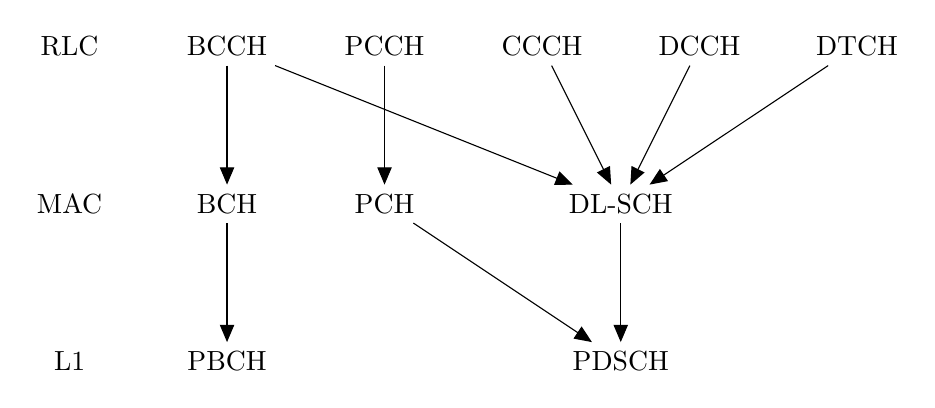
\begin{tikzpicture}[scale=.5]

\node at (-10,5) {RLC};
\node at (-10,1) {MAC};
\node at (-10,-3) {L1};

\node (v1) at (-6,5) {BCCH};
\node (v2) at (-6,1) {BCH};
\node (v3) at (-6,-3) {PBCH};

\node (v5) at (-2,5) {PCCH};
\node (v6) at (-2,1) {PCH};

\node (v8) at (2,5) {CCCH};

\node (v9) at (6,5) {DCCH};

\node (v10) at (10,5) {DTCH};
\node (v4) at (4,1) {DL-SCH};
\node (v7) at (4,-3) {PDSCH};

%\node (v11) at (14,5) {MCCH};
%
%\node (v12) at (18,5) {MTCH};
%\node (v13) at (18,1) {MCH};
%\node (v14) at (18,-3) {PMCH};

\draw [arrows={-triangle 45}] (v1) edge (v2);
\draw [arrows={-triangle 45}] (v2) edge (v3);
\draw [arrows={-triangle 45}] (v1) edge (v4);
\draw [arrows={-triangle 45}] (v5) edge (v6);
\draw [arrows={-triangle 45}] (v6) edge (v7);
\draw [arrows={-triangle 45}] (v8) edge (v4);
\draw [arrows={-triangle 45}] (v9) edge (v4);
\draw [arrows={-triangle 45}] (v10) edge (v4);
\draw [arrows={-triangle 45}] (v4) edge (v7);
%\draw [arrows={-triangle 45}] (v11) edge (v4);
%\draw [arrows={-triangle 45}] (v12) edge (v4);
%\draw [arrows={-triangle 45}] (v12) edge (v13);
%\draw [arrows={-triangle 45}] (v13) edge (v14);
\end{tikzpicture}}
	\caption{\gls{MAC} layer \gls{DL} mapping structure \citep[Sec. 6.3]{book_LTE_for_UMTS}.}
	\label{fig:MAC_PDU_DL}
	\end{figure}
\end{minipage}
\begin{minipage}{0.48\textwidth}
	\tikzsetnextfilename{MAC_UL-mapping}
	\begin{figure}[H]
	\centering
	\resizebox{\textwidth}{!}{
	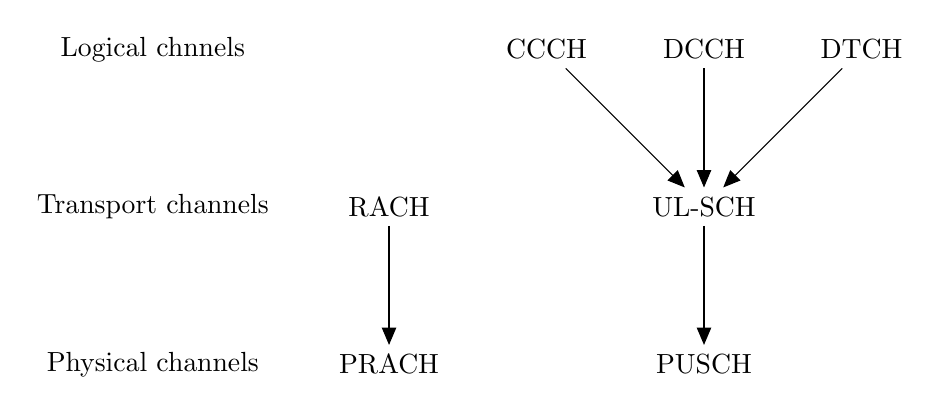
\begin{tikzpicture}[scale=.5]

\node at (-10,5) {Logical chnnels};
\node at (-10,1) {Transport channels};
\node at (-10,-3) {Physical channels};

\node (v1) at (-4,1) {RACH};
\node (v2) at (-4,-3) {PRACH};

\node (v3) at (0,5) {CCCH};

\node (v4) at (4,5) {DCCH};

\node (v5) at (8,5) {DTCH};
\node (v6) at (4,1) {UL-SCH};
\node (v7) at (4,-3) {PUSCH};


\draw [arrows={-triangle 45}] (v1) edge (v2);
\draw [arrows={-triangle 45}] (v3) edge (v6);
 \draw [arrows={-triangle 45}] (v4) edge (v6);
 \draw [arrows={-triangle 45}] (v5) edge (v6);
 \draw [arrows={-triangle 45}] (v6) edge (v7);
\end{tikzpicture}}
	\caption{\gls{MAC} layer \gls{UL} mapping structure \citep[Sec. 6.3]{book_LTE_for_UMTS}.}
	\label{fig:MAC_PDU_UL}
	\end{figure}
\end{minipage}
\captionsetup{belowskip=-1.5em}

A \gls{MAC} \gls{PDU} consist of the \gls{MAC} header, the \gls{MAC} control elements, the \gls{MAC} \gls{SDU}s and potentially some padding as can be seen in \autoref{fig:MAC_PDU}

\tikzsetnextfilename{MAC_PDU}
\begin{figure}[H]
\centering
\resizebox{\textwidth}{!}{
\usetikzlibrary{decorations.pathreplacing}
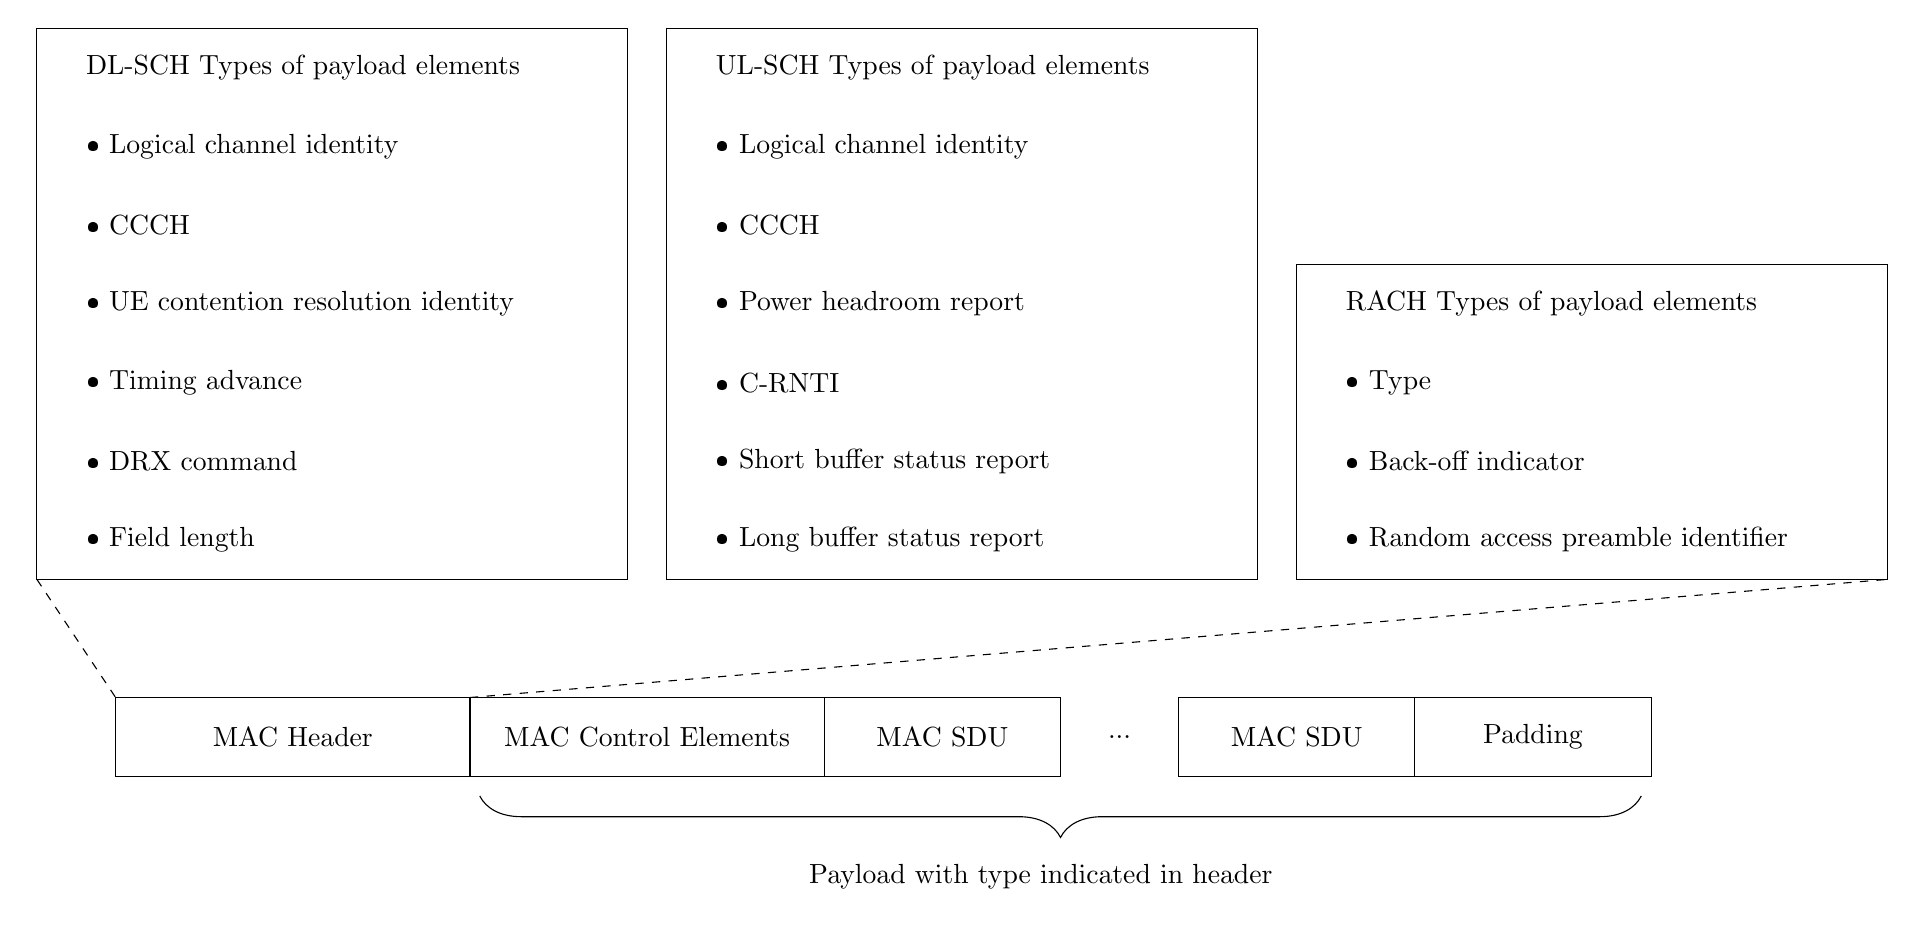
\begin{tikzpicture}[scale=.5]

\draw  (-10,8) rectangle (5,-6);
\node [anchor=west] at (-9,7) {DL-SCH Types of payload elements};
\node [anchor=west] at (-9,5) {• Logical channel identity};
\node [anchor=west] at (-9,3) {• CCCH};
\node [anchor=west] at (-9,1) {• UE contention resolution identity};
\node [anchor=west] at (-9,-1) {• Timing advance};
\node [anchor=west] at (-9,-3) {• DRX command};
\node [anchor=west] at (-9,-5) {• Field length};

\draw  (6,8) rectangle (21,-6) {};
\node [anchor=west] at (7,7) {UL-SCH Types of payload elements};
\node [anchor=west] at (7,5) {• Logical channel identity};
\node [anchor=west] at (7,3) {• CCCH};
\node [anchor=west] at (7,1) {• Power headroom report};
\node [anchor=west] at (7,-1) {• C-RNTI};
\node [anchor=west] at (7,-3) {• Short buffer status report};
\node [anchor=west] at (7,-5) {• Long buffer status report};

\draw  (22,2) rectangle (37,-6) node (v4) {};
\node [anchor=west] at (23,1) {RACH Types of payload elements};
\node [anchor=west] at (23,-1) {• Type};
\node [anchor=west] at (23,-3) {• Back-off indicator};
\node [anchor=west] at (23,-5) {• Random access preamble identifier};

\draw  (-8,-9) node (v2) {} rectangle (1,-11);
\node at (-3.5,-10) {MAC Header};
\draw  (1,-9) node (v3) {} rectangle (10,-11);
\node at (5.5,-10) {MAC Control Elements};
\draw  (10,-9) rectangle (16,-11);
\node at (13,-10) {MAC SDU};
\node at (17.5,-10) {...};
\draw  (19,-9) rectangle (25,-11);
\node at (22,-10) {MAC SDU};
\draw  (25,-9) rectangle (31,-11);
\node at (28,-10) {Padding};

\node (v1) at (-10,-6) {};
\draw [dashed] (-10,-6) -- (-8,-9);
\draw [dashed] (1,-9) -- (37,-6);
\node (v5) at (1,-11.5) {};
\node (v6) at (31,-11.5) {};
\draw [decorate,decoration={brace,amplitude=15pt}] (v6) -- (v5);
\node [anchor=north] at (15.5,-13) {Payload with type indicated in header};
\end{tikzpicture}}
\caption{MAC PDU structure \citep[Sec. 6.3]{book_LTE_for_UMTS}.}
\label{fig:MAC_PDU}
\end{figure}

The header is different depending upon which transport channel is used, as can be seen on \autoref{fig:MAC_PDU}. It include key parameters for control of both the physical layer as well as the logical channel identity. It is also the \gls{MAC} layer that handles contention resolution with \gls{HARQ}, which requires the header to include \gls{CCCH} and \gls{C-RNTI} for the device. When a device tries to connect to the network, the \gls{MAC} layer also calculates timing advance. \citep[Sec. 6.3]{book_LTE_for_UMTS}


\subsection{PHY}\label{sec:NB-IoT/Physical Layer}

To accommodate the new requirements set by the \gls{IoT} development, as described in the beginning of \autoref{ch:NB-IoT}, the physical layer design also needs to be revised. The idea is to allow for three different deployments methods: in-band, guard-band and standalone \citep{primer}. This is to take advantage of the existing \gls{LTE} and \gls{GSM} networks. The idea behind the three deployments can be seen on \autoref{fig:NB deployment}. The in-band mode takes up one of the \gls{PRB} from the \gls{LTE} cell, where the guard-band mode places it just outside the LTE carriers. This is possible because none of the \gls{LTE} cells utilize the entire allocated spectrum to reduce the spectral disturbance. The proposed design also allows for the standalone case to utilize a \gls{GSM} band taking advantage of the lower frequency compared to legacy \gls{LTE} to increase the coverage area. To work inside and alongside these system provides some restrictions that needs to be respected. Therefore is the physical structure of the system the same for all deployment methods, however the use and spectrum allocation differs slightly. The most commonly discussed deployment scenario is the in-band operation as this set the most restriction for the \gls{NB-IoT} system. \citep{REL-13,primer}

\begin{figure}[H]
\centering
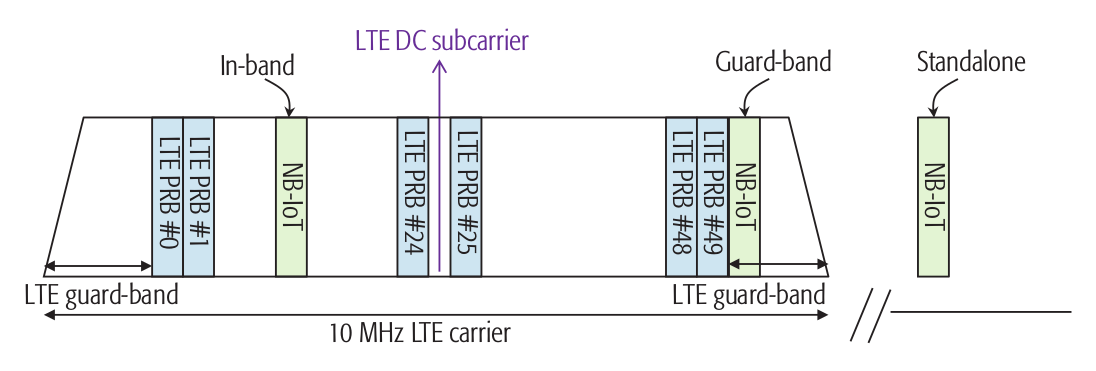
\includegraphics[width=\textwidth]{figures/deployment.png}
\caption{Deployment of the NB-IoT as in-band, guard-band or standalone \citep{primer}.}
\label{fig:NB deployment}
\end{figure}

To allow in-band operation, the physical layer of \gls{NB-IoT} needs to follow the overall structure of \gls{LTE}. To describe this, it is split into the \gls{DL} and \gls{UL} part. First the \gls{DL} part will be investigated as this accounts for most of the critical factors of the communication i.e. synchronization and system information. 

\subsubsection{Downlink}
As the primary users of legacy \gls{LTE} does not know of the \gls{NB-IoT} system, the primary concern is the interference it causes. Some structural guidelines is therefore needed when designing the \gls{NB-IoT} system, here under it needs to blend in with the \gls{OFDM} symbols of the \gls{LTE} system, meaning that timing alignment and subcarrier spacing is already determined \citep[ch. 7.2]{NB-IoT_Book}. 

Channel Raster\\
As \gls{NB-IoT} functions as an individual system, it needs it own overhead. To ensure the functionality of both systems, the \gls{PRB}s used for \gls{NB-IoT} is therefore placed outside the six center \gls{PRB}'s, as these are used for LTE synchronization. This implies that only the LTE cells with a bandwidth larger than 1.4 MHz can host NB-IoT \citep{whitepaper}. Furthermore to keep the receiver complexity and the battery consumption at a minimum, the device searches for the \gls{NB-IoT} cell on a raster of 100 kHz \citep[ch. 7.2]{NB-IoT_Book}. The center of the bandwidth host a DC-subcarrier and the \gls{PRB}'s is placed around this. This means that the center of a PRB will be offset from the raster, for instance PRB \#25 in \autoref{fig:NB deployment} has a center of 97.5 kHz, which is 2.5 kHz off from the raster. Because of this, an additional requirement is made that only those \gls{PRB}'s, where the offset is less than 7.5 kHz can be used to host a NB-IoT cell \citep{primer}. The PRB's that fulfill this criteria can be seen in \autoref{tab:available-PRBs}. 

\begin{table}[H]
\centering
\begin{tabular}{|c|p{1.8cm}|p{1.8cm}|p{1.8cm}|p{1.8cm}|p{1.8cm}|}\hline
\textbf{LTE cell bandwidth}	& 3 MHz				& 5 MHz	& 10 MHz	& 15 MHz	& 20 MHz \\\hline
Available PRB indexes		& 2, 12	& 2, 7, 17, 22	& 4, 9, 14, 19, 30, 35, 40, 45 & 2, 7, 12, 17, 22, 27, 32, 42, 47, 52, 57, 62, 67, 72 & 4, 9, 14, 19, 24, 29, 34, 39, 44, 55, 60, 65, 70, 75, 80, 85, 90, 95 \\\hline
\end{tabular}
\caption{Available PRBs depending on the bandwidth of the LTE cell \citep{whitepaper}.}
\label{tab:available-PRBs}
\end{table}


Frame Structure\\
To fit into a \gls{LTE} \gls{PRB}, the frame structure needs to be very similar to legacy \gls{LTE}. The structure is divided into: hyperframe, frame, subframe and slots. Where two slots make a subframe, ten subframes make a frame and 1024 frames make a hyperframe. A complete cycle takes 1024 hyperframes, which corresponds to 2 hours 54 minutes and 46 seconds. This structure is shown on \autoref{fig:downlink-structure}. \citep[ch. 7.2]{NB-IoT_Book}


\begin{figure}[H]
\centering
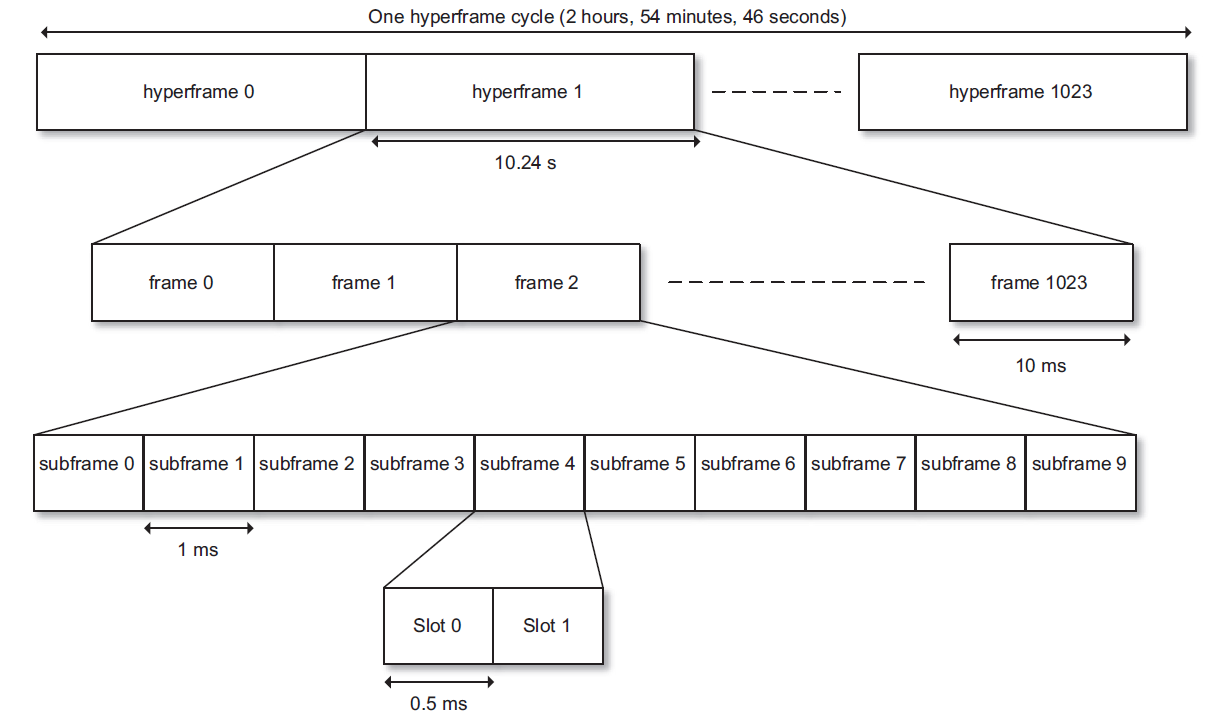
\includegraphics[width=\textwidth]{figures/downlink_structure_15kHz.png}
\caption{\gls{NB-IoT} downlink structure \citep[Fig. 7.7]{NB-IoT_Book}.}
\label{fig:downlink-structure}
\end{figure}


As the \gls{NB-IoT} system is placed outside the \gls{PRB}s used for LTE synchronization, most of the subframes are available to use, with the only exception being when a \gls{MBSFN} is present, which can occupy either of subframes (1,2,3,6,7,8) \citep{LTE-MBSFN}. Therefore the \gls{NPSS} and \gls{NSSS} is placed in subframe 5 and 9 respectively as seen on \autoref{fig:frame-structure}. By having the \gls{NSSS} being present only in even numbered frame, the \gls{LSB} of the frame numbers can be deduced directly. This increases the efficiency of the system by freeing subframe 9 in odd numbered frames and omitting that bit from the \gls{NB-IoT} overhead. The \gls{NPBCH} is located in the subframe 0 and contains the \gls{MIB-NB} \citep{REL-13}.  

\tikzsetnextfilename{frameStructure}
\begin{figure}[H]
\centering
\definecolor{NPSS}{HTML}{00D0FF}
\definecolor{NSSS}{HTML}{F97BFF}
\definecolor{NPBCH}{HTML}{92D050}
\usetikzlibrary{patterns,decorations.pathreplacing}

\resizebox{\textwidth}{!}{
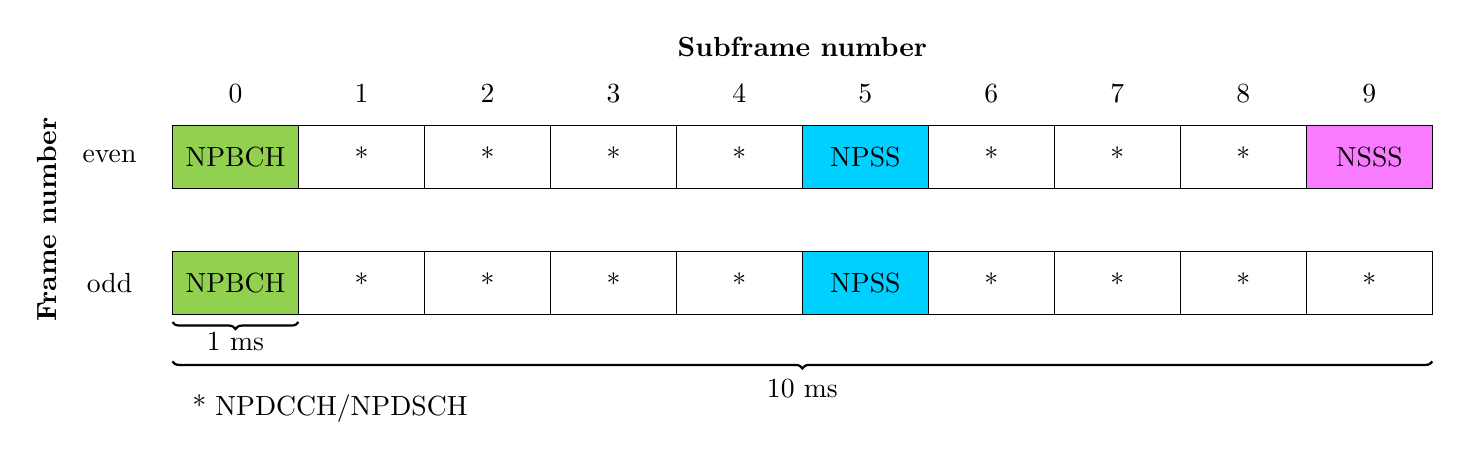
\begin{tikzpicture}[scale = 0.4]

\draw [thick,decoration={brace,mirror,raise=0.1cm},decorate] (-20,-4) -- (-16,-4) node [pos=0.5,anchor=north,yshift=-0.1cm] {1 ms}; 
\draw [thick,decoration={brace,mirror,raise=0.2cm},decorate] (-20,-5) -- (20,-5) node [pos=0.5,anchor=north,yshift=-0.3cm] {10 ms};



\draw[fill = NPBCH]  (-20,2) rectangle (-16,0);
\draw  (-16,2) rectangle (-12,0);
\draw  (-12,2) rectangle (-8,0);
\draw  (-8,2) rectangle (-4,0);
\draw  (-4,2) rectangle (0,0);
\draw[fill = NPSS]  (0,2) rectangle (4,0);
\draw  (4,2) rectangle (8,0);
\draw  (8,2) rectangle (12,0);
\draw  (12,2) rectangle (16,0);
\draw[fill = NSSS]  (16,2) rectangle (20,0);

\draw[fill = NPBCH]  (-20,-2) rectangle (-16,-4);
\draw  (-16,-2) rectangle (-12,-4);
\draw  (-12,-2) rectangle (-8,-4);
\draw  (-8,-2) rectangle (-4,-4);
\draw  (-4,-2) rectangle (0,-4);
\draw[fill = NPSS]  (0,-2) rectangle (4,-4);
\draw  (4,-2) rectangle (8,-4);
\draw  (8,-2) rectangle (12,-4);
\draw  (12,-2) rectangle (16,-4);
\draw  (16,-2) rectangle (20,-4);

\node at (-18,3) {0};
\node at (-14,3) {1};
\node at (-10,3) {2};
\node at (-6,3) {3};
\node at (-2,3) {4};
\node at (2,3) {5};
\node at (6,3) {6};
\node at (10,3) {7};
\node at (14,3) {8};
\node at (18,3) {9};
\node at (-22,1) {even};
\node at (-22,-3) {odd};
\node [rotate = 90] at (-24,-1) {\textbf{Frame number}}; 

\node at (-18,1) {\acrshort{NPBCH}};
\node at (-18,-3) {\acrshort{NPBCH}};
\node at (2,1) {\acrshort{NPSS}};
\node at (2,-3) {\acrshort{NPSS}};
\node at (18,1) {\acrshort{NSSS}};
\node at (-14,1) {*};
\node at (-10,1) {*};
\node at (-6,1) {*};
\node at (-2,1) {*};
\node at (6,1) {*};
\node at (10,1) {*};
\node at (14,1) {*};
\node at (-14,-3) {*};
\node at (-10,-3) {*};
\node at (-6,-3) {*};
\node at (-2,-3) {*};
\node at (6,-3) {*};
\node at (10,-3) {*};
\node at (14,-3) {*};
\node at (18,-3) {*};
\node at (0,4.5) {\textbf{Subframe number}}; 

\node at (-15,-7) {* \acrshort{NPDCCH}/\acrshort{NPDSCH}};
\end{tikzpicture}
}

\caption{\gls{NB-IoT} frame structure \citep{REL-13}.}
\label{fig:frame-structure}
\end{figure}


By zooming in on a subframe, it is possible to see how the different \gls{OFDM} symbols is utilized. During a subframe, 14 \gls{OFDM} symbols are transmitted, each having 12 subcarriers, which results in 168 \gls{RE} per subframe. As can be seen on \autoref{fig:subframe-structure}, almost half of the \gls{RE} in a subframe might be reserved for different signals and \gls{LTE} control information \citep{REL-13}. An \gls{LTE} cell can allocate up to three symbols for \gls{PDCCH} and might use up to four carrier, which needs four \gls{RS}s \citep{whitepaper}. The \gls{NB-IoT} structure allows for up to two carriers and needs therefore two \gls{RS} namely \gls{NRS}1 and \gls{NRS}2 \citep{REL-13}. The placement of all these signals can be seen in \autoref{fig:subframe-structure}.  

\tikzsetnextfilename{subframe}
\begin{figure}[H]
\centering
\definecolor{LTERS}{HTML}{496d22}
\definecolor{LTECCH}{HTML}{92D050}
\definecolor{NPSS}{HTML}{00D0FF}
\definecolor{NSSS}{HTML}{F97BFF}


\resizebox{\textwidth}{!}{
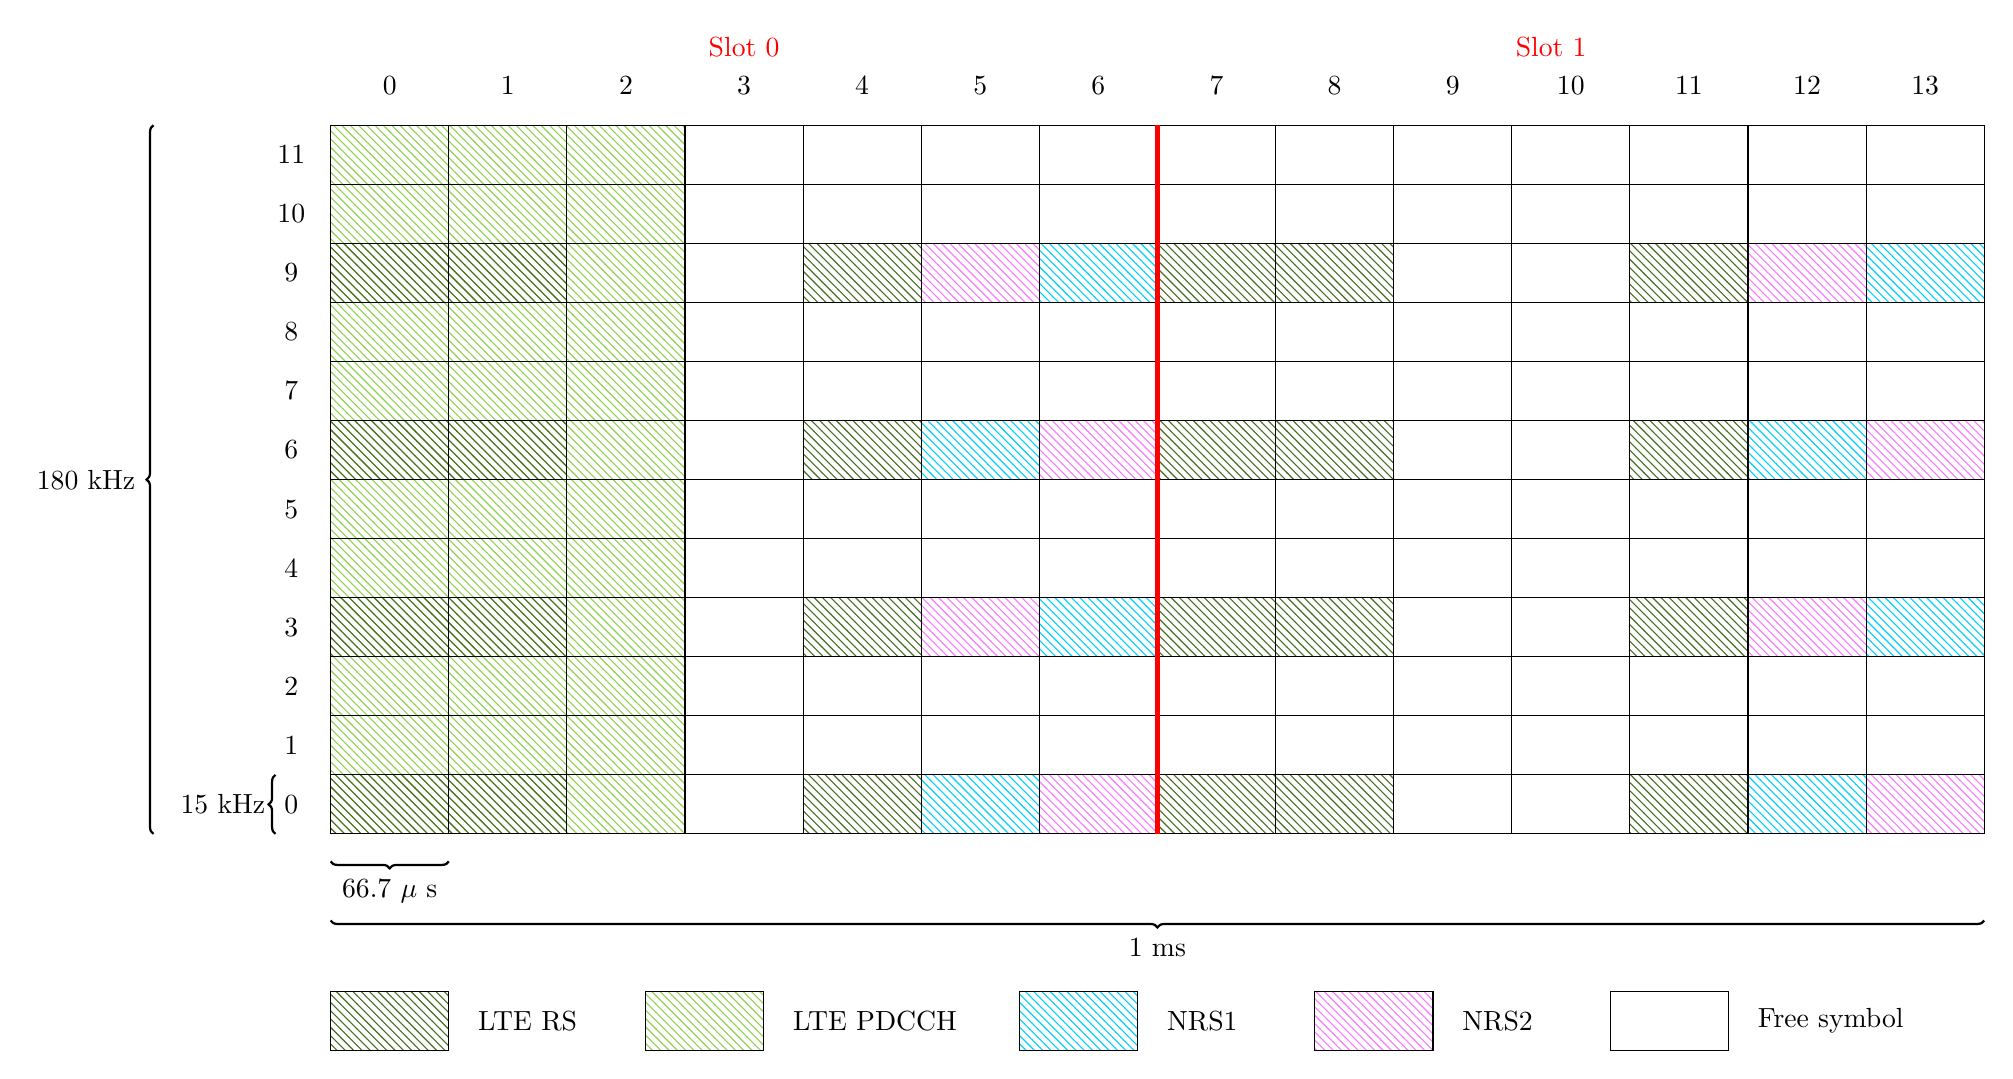
\begin{tikzpicture}[scale=0.5]

\draw[pattern=north west lines, pattern color=LTECCH]  (-21,9) rectangle (-12,-9);
\draw [thick,decoration={brace,mirror},decorate] (-25.5,9) -- (-25.5,-9) node [pos=0.5,anchor=east, xshift=-0.1cm] {180 kHz};
\draw [thick,decoration={brace,mirror,raise=0.1cm},decorate] (-22.2,-7.5) -- (-22.2,-9) node [pos=0.5,anchor=east,xshift=-0.1cm] {15 kHz};
\draw [thick,decoration={brace,mirror,raise=0.1cm},decorate] (-21,-9.5) -- (-18,-9.5) node [pos=0.5,anchor=north,yshift=-0.2cm] {66.7 $\mu$ s};
\draw [thick,decoration={brace,mirror,raise=0.1cm},decorate] (-21,-11) -- (21,-11) node [pos=0.5,anchor=north,yshift=-0.2cm] {1 ms};


\node[text =red] at (-10.5,11) {Slot 0};
\node[text =red] at (10,11) {Slot 1};

%række 11
\draw  (-21,9) rectangle (-18,7.5);
\draw  (-18,9) rectangle (-15,7.5);
\draw  (-15,9) rectangle (-12,7.5);
\draw  (-12,9) rectangle (-9,7.5);
\draw  (-9,9) rectangle (-6,7.5);
\draw  (-6,9) rectangle (-3,7.5);
\draw  (-3,9) rectangle (0,7.5);
\draw  (-0,9) node (v1) {} rectangle (3,7.5);
\draw  (3,9) rectangle (6,7.5);
\draw  (6,9) rectangle (9,7.5);
\draw  (9,9) rectangle (12,7.5);
\draw  (12,9) rectangle (15,7.5);
\draw  (15,9) rectangle (18,7.5);
\draw  (18,9) rectangle (21,7.5);

%række 10
\draw  (-21,7.5) rectangle (-18,6);
\draw  (-18,7.5) rectangle (-15,6);
\draw  (-15,7.5) rectangle (-12,6);
\draw  (-12,7.5) rectangle (-9,6);
\draw  (-9,7.5) rectangle (-6,6);
\draw  (-6,7.5) rectangle (-3,6);
\draw  (-3,7.5) rectangle (0,6);
\draw  (-0,7.5) rectangle (3,6);
\draw  (3,7.5) rectangle (6,6);
\draw  (6,7.5) rectangle (9,6);
\draw  (9,7.5) rectangle (12,6);
\draw  (12,7.5) rectangle (15,6);
\draw  (15,7.5) rectangle (18,6);
\draw  (18,7.5) rectangle (21,6);

%række 9
\draw[pattern=north west lines, pattern color=LTERS] (-21,6) rectangle (-18,4.5);
\draw[pattern=north west lines, pattern color=LTERS] (-18,6) rectangle (-15,4.5);
\draw  (-15,6) rectangle (-12,4.5);
\draw  (-12,6) rectangle (-9,4.5);
\draw[pattern=north west lines, pattern color=LTERS]  (-9,6) rectangle (-6,4.5);
\draw[pattern=north west lines, pattern color=NSSS]  (-6,6) rectangle (-3,4.5);
\draw[pattern=north west lines, pattern color=NPSS]  (-3,6) rectangle (0,4.5);
\draw[pattern=north west lines, pattern color=LTERS]  (-0,6) rectangle (3,4.5);
\draw[pattern=north west lines, pattern color=LTERS]  (3,6) rectangle (6,4.5);
\draw  (6,6) rectangle (9,4.5);
\draw  (9,6) rectangle (12,4.5);
\draw[pattern=north west lines, pattern color=LTERS]  (12,6) rectangle (15,4.5);
\draw[pattern=north west lines, pattern color=NSSS] (15,6) rectangle (18,4.5);
\draw[pattern=north west lines, pattern color=NPSS]  (18,6) rectangle (21,4.5);

%række 8
\draw  (-21,4.5) rectangle (-18,3);
\draw  (-18,4.5) rectangle (-15,3);
\draw  (-15,4.5) rectangle (-12,3);
\draw  (-12,4.5) rectangle (-9,3);
\draw  (-9,4.5) rectangle (-6,3);
\draw  (-6,4.5) rectangle (-3,3);
\draw  (-3,4.5) rectangle (0,3);
\draw  (-0,4.5) rectangle (3,3);
\draw  (3,4.5) rectangle (6,3);
\draw  (6,4.5) rectangle (9,3);
\draw  (9,4.5) rectangle (12,3);
\draw  (12,4.5) rectangle (15,3);
\draw  (15,4.5) rectangle (18,3);
\draw  (18,4.5) rectangle (21,3);

%række 7
\draw  (-21,3) rectangle (-18,1.5);
\draw  (-18,3) rectangle (-15,1.5);
\draw  (-15,3) rectangle (-12,1.5);
\draw  (-12,3) rectangle (-9,1.5);
\draw  (-9,3) rectangle (-6,1.5);
\draw  (-6,3) rectangle (-3,1.5);
\draw  (-3,3) rectangle (0,1.5);
\draw  (-0,3) rectangle (3,1.5);
\draw  (3,3) rectangle (6,1.5);
\draw  (6,3) rectangle (9,1.5);
\draw  (9,3) rectangle (12,1.5);
\draw  (12,3) rectangle (15,1.5);
\draw  (15,3) rectangle (18,1.5);
\draw  (18,3) rectangle (21,1.5);

%række 6
\draw[pattern=north west lines, pattern color=LTERS] (-21,1.5) rectangle (-18,0);
\draw[pattern=north west lines, pattern color=LTERS] (-18,1.5) rectangle (-15,0);
\draw  (-15,1.5) rectangle (-12,0);
\draw  (-12,1.5) rectangle (-9,0);
\draw[pattern=north west lines, pattern color=LTERS]  (-9,1.5) rectangle (-6,0);
\draw[pattern=north west lines, pattern color=NPSS]  (-6,1.5) rectangle (-3,0);
\draw[pattern=north west lines, pattern color=NSSS]  (-3,1.5) rectangle (0,0);
\draw[pattern=north west lines, pattern color=LTERS]  (-0,1.5) rectangle (3,0);
\draw[pattern=north west lines, pattern color=LTERS]  (3,1.5) rectangle (6,0);
\draw  (6,1.5) rectangle (9,0);
\draw  (9,1.5) rectangle (12,0);
\draw[pattern=north west lines, pattern color=LTERS]  (12,1.5) rectangle (15,0);
\draw[pattern=north west lines, pattern color=NPSS]  (15,1.5) rectangle (18,0);
\draw[pattern=north west lines, pattern color=NSSS] (18,1.5) rectangle (21,0);

%række 5
\draw  (-21,-0) rectangle (-18,-1.5);
\draw  (-18,-0) rectangle (-15,-1.5);
\draw  (-15,-0) rectangle (-12,-1.5);
\draw  (-12,-0) rectangle (-9,-1.5);
\draw  (-9,-0) rectangle (-6,-1.5);
\draw  (-6,-0) rectangle (-3,-1.5);
\draw  (-3,-0) rectangle (0,-1.5);
\draw  (-0,-0) rectangle (3,-1.5);
\draw  (3,-0) rectangle (6,-1.5);
\draw  (6,-0) rectangle (9,-1.5);
\draw  (9,-0) rectangle (12,-1.5);
\draw  (12,-0) rectangle (15,-1.5);
\draw  (15,-0) rectangle (18,-1.5);
\draw  (18,-0) rectangle (21,-1.5);

%række 4
\draw  (-21,-1.5) rectangle (-18,-3);
\draw  (-18,-1.5) rectangle (-15,-3);
\draw  (-15,-1.5) rectangle (-12,-3);
\draw  (-12,-1.5) rectangle (-9,-3);
\draw  (-9,-1.5) rectangle (-6,-3);
\draw  (-6,-1.5) rectangle (-3,-3);
\draw  (-3,-1.5) rectangle (0,-3);
\draw  (-0,-1.5) rectangle (3,-3);
\draw  (3,-1.5) rectangle (6,-3);
\draw  (6,-1.5) rectangle (9,-3);
\draw  (9,-1.5) rectangle (12,-3);
\draw  (12,-1.5) rectangle (15,-3);
\draw  (15,-1.5) rectangle (18,-3);
\draw  (18,-1.5) rectangle (21,-3);

%række 3
\draw[pattern=north west lines, pattern color=LTERS] (-21,-3) rectangle (-18,-4.5);
\draw[pattern=north west lines, pattern color=LTERS] (-18,-3) rectangle (-15,-4.5);
\draw  (-15,-3) rectangle (-12,-4.5);
\draw  (-12,-3) rectangle (-9,-4.5);
\draw[pattern=north west lines, pattern color=LTERS]  (-9,-3) rectangle (-6,-4.5);
\draw[pattern=north west lines, pattern color=NSSS]  (-6,-3) rectangle (-3,-4.5);
\draw[pattern=north west lines, pattern color=NPSS]  (-3,-3) rectangle (0,-4.5);
\draw[pattern=north west lines, pattern color=LTERS]  (-0,-3) rectangle (3,-4.5);
\draw[pattern=north west lines, pattern color=LTERS]  (3,-3) rectangle (6,-4.5);
\draw  (6,-3) rectangle (9,-4.5);
\draw  (9,-3) rectangle (12,-4.5);
\draw[pattern=north west lines, pattern color=LTERS]  (12,-3) rectangle (15,-4.5);
\draw[pattern=north west lines, pattern color=NSSS]  (15,-3) rectangle (18,-4.5);
\draw[pattern=north west lines, pattern color=NPSS]  (18,-3) rectangle (21,-4.5);

%række 2
\draw  (-21,-4.5) rectangle (-18,-6);
\draw  (-18,-4.5) rectangle (-15,-6);
\draw  (-15,-4.5) rectangle (-12,-6);
\draw  (-12,-4.5) rectangle (-9,-6);
\draw  (-9,-4.5) rectangle (-6,-6);
\draw  (-6,-4.5) rectangle (-3,-6);
\draw  (-3,-4.5) rectangle (0,-6);
\draw  (-0,-4.5) rectangle (3,-6);
\draw  (3,-4.5) rectangle (6,-6);
\draw  (6,-4.5) rectangle (9,-6);
\draw  (9,-4.5) rectangle (12,-6);
\draw  (12,-4.5) rectangle (15,-6);
\draw  (15,-4.5) rectangle (18,-6);
\draw  (18,-4.5) rectangle (21,-6);

%række 1
\draw  (-21,-6) rectangle (-18,-7.5);
\draw  (-18,-6) rectangle (-15,-7.5);
\draw  (-15,-6) rectangle (-12,-7.5);
\draw  (-12,-6) rectangle (-9,-7.5);
\draw  (-9,-6) rectangle (-6,-7.5);
\draw  (-6,-6) rectangle (-3,-7.5);
\draw  (-3,-6) rectangle (0,-7.5);
\draw  (-0,-6) rectangle (3,-7.5);
\draw  (3,-6) rectangle (6,-7.5);
\draw  (6,-6) rectangle (9,-7.5);
\draw  (9,-6) rectangle (12,-7.5);
\draw  (12,-6) rectangle (15,-7.5);
\draw  (15,-6) rectangle (18,-7.5);
\draw  (18,-6) rectangle (21,-7.5);

%række 0
\draw[pattern=north west lines, pattern color=LTERS] (-21,-7.5) rectangle (-18,-9);
\draw[pattern=north west lines, pattern color=LTERS] (-18,-7.5) rectangle (-15,-9);
\draw  (-15,-7.5) rectangle (-12,-9); 
\draw  (-12,-7.5) rectangle (-9,-9);
\draw[pattern=north west lines, pattern color=LTERS]  (-9,-7.5) rectangle (-6,-9);
\draw[pattern=north west lines, pattern color=NPSS]  (-6,-7.5) rectangle (-3,-9);
\draw[pattern=north west lines, pattern color=NSSS]  (-3,-7.5) rectangle (0,-9) node (v2) {};
\draw[pattern=north west lines, pattern color=LTERS]  (-0,-7.5) rectangle (3,-9);
\draw[pattern=north west lines, pattern color=LTERS]  (3,-7.5) rectangle (6,-9);
\draw  (6,-7.5) rectangle (9,-9);
\draw  (9,-7.5) rectangle (12,-9);
\draw[pattern=north west lines, pattern color=LTERS]  (12,-7.5) rectangle (15,-9);
\draw[pattern=north west lines, pattern color=NPSS]  (15,-7.5) rectangle (18,-9);
\draw[pattern=north west lines, pattern color=NSSS]  (18,-7.5) rectangle (21,-9);


\node at (-22,-8.25) {0};
\node at (-22,-6.75) {1};
\node at (-22,-5.25) {2};
\node at (-22,-3.75) {3};
\node at (-22,-2.25) {4};
\node at (-22,-0.75) {5};
\node at (-22,0.75) {6};
\node at (-22,2.25) {7};
\node at (-22,3.75) {8};
\node at (-22,5.25) {9};
\node at (-22,6.75) {10};
\node at (-22,8.25) {11};

\node at (-19.5,10) {0};
\node at (-16.5,10) {1};
\node at (-13.5,10) {2};
\node at (-10.5,10) {3};
\node at (-7.5,10) {4};
\node at (-4.5,10) {5};
\node at (-1.5,10) {6};
\node at (1.5,10) {7};
\node at (4.5,10) {8};
\node at (7.5,10) {9};
\node at (10.5,10) {10};
\node at (13.5,10) {11};
\node at (16.5,10) {12};
\node at (19.5,10) {13};

\draw[draw=red,line width=2pt] (0,9) -- (0,-9);
\draw[pattern=north west lines, pattern color=LTERS]  (-21,-13) rectangle (-18,-14.5);
\draw[pattern=north west lines, pattern color=LTECCH]  (-13,-13) rectangle (-10,-14.5);
\draw[pattern=north west lines, pattern color=NPSS]  (-3.5,-13) rectangle (-0.5,-14.5) ;
\draw[pattern=north west lines, pattern color=NSSS]  (4,-13) rectangle (7,-14.5) ;
\draw (11.5,-13) rectangle (14.5,-14.5);

\node[anchor=west] at (-17.5,-13.75) {\acrshort{LTE} \acrshort{RS}};
\node[anchor=west] at (-9.5,-13.75) {\acrshort{LTE} \acrshort{PDCCH}};
\node[anchor=west] at (-0,-13.75) {\acrshort{NRS}1};
\node[anchor=west] at (7.5,-13.75) {\acrshort{NRS}2};
\node[anchor=west] at (15,-13.75) {Free symbol};

\end{tikzpicture}
}
\caption{The structure of a \gls{DL} subframe \citep{whitepaper,REL-13}.}
\label{fig:subframe-structure}
\end{figure}

It should be noted that the described allocation is a worst case scenario for the \gls{DL}. If the system is deployed either in guard-band or as stand-alone, only the \gls{NRS} is actually used, but before the device is synchronized, it does not know what is in use and needs to guard for this worst case scenario. When the device receives the \gls{MIB-NB} and \gls{NB-SIB}1 it will get information in regards to the number of carriers and the size of \gls{LTE} \gls{PDCCH} \citep{whitepaper}. 

Channels\\ 
As shown on \autoref{fig:frame-structure}, three channels exist in the physical \gls{DL} part of the protocol. These are respectively: \gls{NPBCH}, \gls{NPDCCH} and \gls{NPDSCH}. The structure of the \gls{NPBCH} is explained in the \autoref{sec:Network_access}.

The \gls{NPDCCH} carries three types of information: one is use to indicate \gls{DL} scheduling for the devices, one provides \gls{UL} grant information and the last indicates paging or system information update \citep{NB-IoT_Book}. It should be noted that  depending on the coverage level the \gls{NPDCCH} might be repeated up 2048 times \citep{NB-IoT_Book}.

The \gls{NPDSCH} is used to transmit data when an bearer is established. Depending on the coverage level the \gls{NPDSCH} might be repeated up 2048 times. A \gls{TBS} may be up to 680 bits depending on the \gls{TBS} index and the number of subframes used. \citep{NB-IoT_Book}

\subsubsection{Uplink}
\label{sec:ULphy}
As mentioned in \autoref{ch:Introduction}, most of the data in the system is \gls{UL} data. Therefore is the \gls{UL} spectrum tuned to accommodate the massive number of devices. The timing alignment of the \gls{UL} follows the \gls{DL} meaning when synchronized to the \gls{DL} band, the device is also synchronized to the \gls{UL}, except for the delay introduced by the travelling time of the signal. This delay is found at the beginning of the \gls{RAP}, which will be further explained in \autoref{sec:RAP}. 

Frame Structure\\
Compared to legacy \gls{LTE}, two differences should be noted. The channel \gls{PUCCH} has been removed and the \gls{UL} frame can take different formats. It is 180 kHz wide, as the \gls{DL} frame, however the sub carrier spacing can be both 3.75 kHz and 15 kHz, giving 48 and 12 subcarriers respectively. This is however only done on the \gls{NPUSCH}, in the \gls{NPRACH} the subcarrier spacing is always 3.75 kHz \citep{NB-IoT_Book}. For each symbol that is transmitted, a \gls{CP} is used. The structure of the channels can be seen on \autoref{fig:NPUSCH1_structure}, \autoref{fig:NPUSCH2_structure} and \autoref{fig:NPRACH_structure}.

\begin{minipage}{0.48\textwidth}
\begin{figure}[H]
\centering
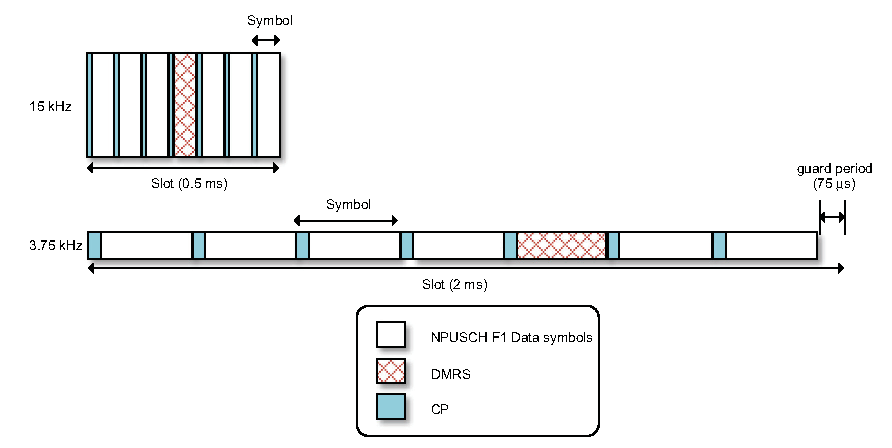
\includegraphics[width=\textwidth]{figures/NPUSCH1_structure.pdf}
\caption{The structure of NPUSCH format 1 \citep{NB-IoT_Book}}
\label{fig:NPUSCH1_structure}
\end{figure}
\end{minipage}%
\hfill
\begin{minipage}{0.48\textwidth}
\begin{figure}[H]
\centering
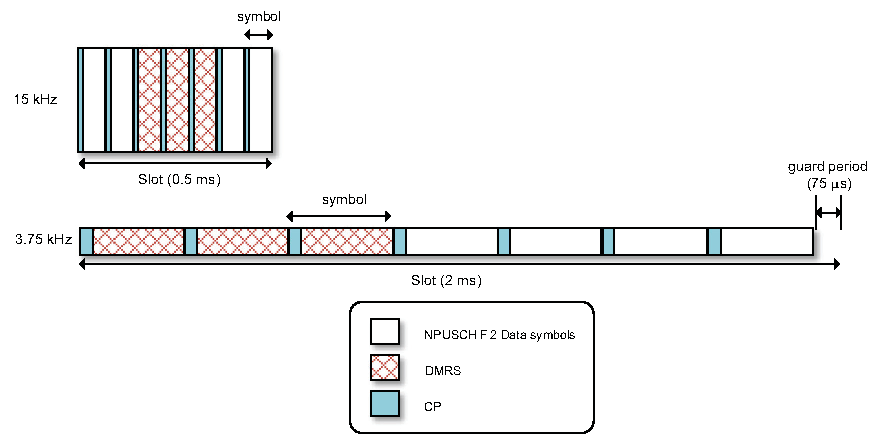
\includegraphics[width=\textwidth]{figures/NPUSCH2_structure.pdf}
\caption{The structure of NPUSCH format 2 \citep{NB-IoT_Book}}
\label{fig:NPUSCH2_structure}
\end{figure}
\end{minipage}


\begin{figure}[H]
\centering
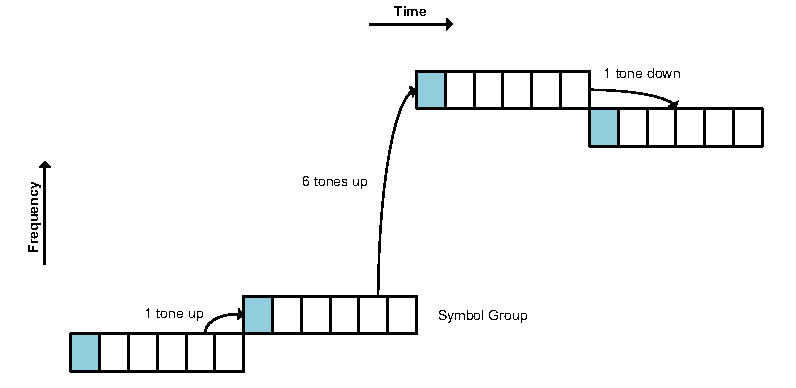
\includegraphics[width=0.5\textwidth]{figures/NPRACH_frequency_hopping.pdf}
\caption{The structure of a NPRACH symbol group \citep{NB-IoT_Book}}
\label{fig:NPRACH_structure}
\end{figure}

Channels\\
The \gls{UL} consists of two channels and one signal, namely the \gls{NPRACH}, \gls{NPUSCH} and \gls{DMRS}.

The \gls{NPRACH} consist of a repetition of four symbol groups, for each symbol group a \gls{CP} is attached followed by five symbols. The duration of the CP is dependent on the CP-format chosen this can be seen in \autoref{fig:NPRACH_structure}, and depending on the coverage level the \gls{NPRACH} might be repeated up to 128 times. The NPRACH only uses 12 subcarriers at any time, which are used for msg1 in the \gls{NRAP}, see \autoref{sec:RAP}. \citep{NB-IoT_Book}

The \gls{NPUSCH} carries the data transmitted form the device and \gls{HARQ} acknowledgement from the \gls{NPDSCH}, this is referred to as format 1 and 2 respectively. Format 1 can carry up 1000 bits per \gls{TB}. As seen on \autoref{fig:NPUSCH1_structure} and \autoref{fig:NPUSCH2_structure} the DMRS, which is used for channel estimation at the base station, is multiplexed with the NPUSCH. 






\section{Network Access}
\label{sec:Network_access}
This section describes the different procedures needed to navigate in the NB-IoT framework. This is the procedure to establish a connection as well as the procedures to navigate between different connection states. 

\subsection{Cell Search and Synchronization Procedure}
\label{sec:cellsync}
The first thing needed for a device is to locate a cell, which is done based on the NPSS and NSSS, mentioned in \autoref{sec:NB-IoT/Physical Layer}. The synchronization procedure is very similar to that of \gls{LTE}, as can be seen on \autoref{fig:sync-NB}, as the device first needs to search for the cell and then acquire the system information. 


\tikzsetnextfilename{sync-NB}
\begin{figure}[H]
\centering
\definecolor{top}{HTML}{00FFFF}
\definecolor{center}{HTML}{0080FF}
\definecolor{bund}{HTML}{0000FF}
\usetikzlibrary{arrows}

%\resizebox{0.5\textwidth}{!}{
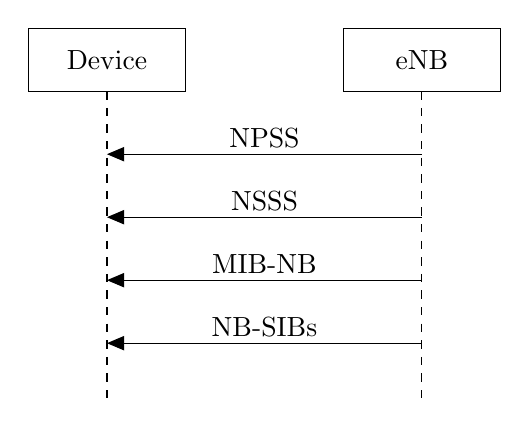
\begin{tikzpicture}[scale = 0.4]

\draw (-7.5,8) rectangle (-2.5,6);
\node at (-5,7) {Device};
\draw [dashed] (-5,6) -- (-5,-4);

\draw (2.5,8) rectangle (7.5,6);
\node at (5,7) {\acrshort{eNB}};
\draw [dashed] (5,6) -- (5,-4);

\draw[arrows={triangle 45-}] (-5,4) -- (5,4);
\node at (0,4.5) {\acrshort{NPSS}};

\draw[arrows={triangle 45-}] (-5,2) -- (5,2);
\node at (0,2.5) {\acrshort{NSSS}};

\draw[arrows={triangle 45-}] (-5,0) -- (5,0);
\node at (0,0.5) {\acrshort{MIB-NB}};

\draw[arrows={triangle 45-}] (-5,-2) -- (5,-2);
\node at (0,-1.5) {\acrshort{NB-SIB}s};

\end{tikzpicture}
%}

\caption{The process needed to synchronize to a cell.}
\label{fig:sync-NB}
\end{figure}

The device first looks for the \gls{NPSS}, where the search spaces are predetermined based on the LTE bands \citep{whitepaper}. This provides the initial \gls{CFO} as well as a 10 ms timing alignment. As mentioned before, the NPSS is located in subframe 5 of each frame. A frequency domain Zadoff-Chu sequence is used for the 11 available \gls{OFDM} symbols, as the first 3 OFDM symbols might be used for LTE PDCCH. For low complexity devices a single 10 ms segment might not suffice at a low \gls{SNR}, so the structure of the \gls{NPSS} is therefore made such that the signals can accumulate coherently over multiple 10 ms segments \citep{NB-IoT_Book,primer}. The \gls{NSSS} is also based on a frequency domain Zadoff-Chu sequence but is further scrambled based on the \gls{NB-PCID}. This means the device has to manually try each frequency and then manually test for each of the 504 NB-PCIDs. When this is done, the device will be synchronized with the eNB, in frequency and time within an 80 ms window and know the NB-PCID also \citep{NB-IoT_Book,primer}. 

The next step is to decode the \gls{MIB-NB}, which consists of 34 bits and 16 \gls{CRC} bits. The MIB-NB is transmitted in the NPBCH in eight self-decodable blocks, which is repeated eight times resulting in a total transmission time of 640 ms as can be seen on \autoref{fig:MIB-NB}. 
 
\tikzsetnextfilename{MIB-NB}
\begin{figure}[H]
\centering
\definecolor{top}{HTML}{00FFFF}
\definecolor{center}{HTML}{0080FF}
\definecolor{bund}{HTML}{0000FF}
\usetikzlibrary{arrows}

\resizebox{\textwidth}{!}{
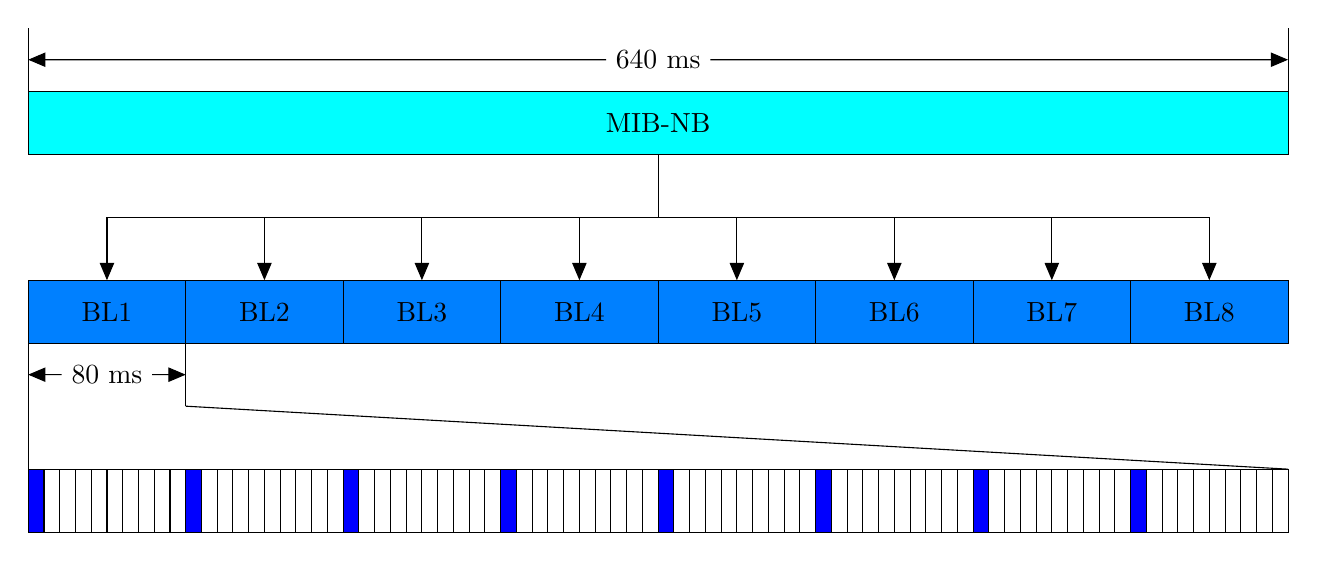
\begin{tikzpicture}[scale = 0.4]

\draw [fill=top] (-20,8) rectangle (20,6);
\node at (0,7) {\acrshort{MIB-NB}};
\draw (-20,10) -- (-20,8);
\draw (20,10) -- (20,8);
\node (top) at (0,9) {640 ms};
\draw[arrows={-triangle 45}] (top) edge (-20,9);
\draw[arrows={-triangle 45}] (top) edge (20,9);

\draw (0,6) -- (0,4); 
\draw (-17.5,4) -- (17.5,4);

\draw[arrows={-triangle 45}] (-17.5,4) -- (-17.5,2);
\draw[arrows={-triangle 45}] (-12.5,4) -- (-12.5,2);
\draw[arrows={-triangle 45}] (-7.5,4) -- (-7.5,2);
\draw[arrows={-triangle 45}] (-2.5,4) -- (-2.5,2);
\draw[arrows={-triangle 45}] (2.5,4) -- (2.5,2);
\draw[arrows={-triangle 45}] (7.5,4) -- (7.5,2);
\draw[arrows={-triangle 45}] (12.5,4) -- (12.5,2);
\draw[arrows={-triangle 45}] (17.5,4) -- (17.5,2);

\draw [fill=center] (-20,2) rectangle (-15,0);
\draw [fill=center] (-15,2) rectangle (-10,0);
\draw [fill=center] (-10,2) rectangle (-5,0);
\draw [fill=center] (-5,2) rectangle (0,0);
\draw [fill=center] (0,2) rectangle (5,0);
\draw [fill=center] (5,2) rectangle (10,0);
\draw [fill=center] (10,2) rectangle (15,0);
\draw [fill=center] (15,2) rectangle (20,0);

\node at (-17.5,1) {BL1};
\node at (-12.5,1) {BL2};
\node at (-7.5,1) {BL3};
\node at (-2.5,1) {BL4};
\node at (2.5,1) {BL5};
\node at (7.5,1) {BL6};
\node at (12.5,1) {BL7};
\node at (17.5,1) {BL8};

\node(bl1) at (-17.5,-1) {80 ms};
\draw[arrows={-triangle 45}] (bl1) edge (-20,-1);
\draw[arrows={-triangle 45}] (bl1) edge (-15,-1);
\draw (-15,0) -- (-15,-2);
\draw (-20,0) -- (-20,-4);
\draw (-15,-2) -- (20,-4);

\draw [fill=bund] (-20,-4) rectangle (-19.5,-6);
\draw [fill=bund] (-15,-4) rectangle (-14.5,-6);
\draw [fill=bund] (-10,-4) rectangle (-9.5,-6);
\draw [fill=bund] (-5,-4) rectangle (-4.5,-6);
\draw [fill=bund] (0,-4) rectangle (0.5,-6);
\draw [fill=bund] (5,-4) rectangle (5.5,-6);
\draw [fill=bund] (10,-4) rectangle (10.5,-6);
\draw [fill=bund] (15,-4) rectangle (15.5,-6);

\draw (-19.5,-4) rectangle (-19,-6);
\draw (-19,-4) rectangle (-18.5,-6);
\draw (-18.5,-4) rectangle (-18,-6);
\draw (-18,-4) rectangle (-17.5,-6);
\draw (-17.5,-4) rectangle (-17,-6);
\draw (-17,-4) rectangle (-16.5,-6);
\draw (-16.5,-4) rectangle (-16,-6);
\draw (-16,-4) rectangle (-15.5,-6);
\draw (-15.5,-4) rectangle (-15,-6);

\draw (-14.5,-4) rectangle (-14,-6);
\draw (-14,-4) rectangle (-13.5,-6);
\draw (-13.5,-4) rectangle (-13,-6);
\draw (-13,-4) rectangle (-12.5,-6);
\draw (-12.5,-4) rectangle (-12,-6);
\draw (-12,-4) rectangle (-11.5,-6);
\draw (-11.5,-4) rectangle (-11,-6);
\draw (-11,-4) rectangle (-10.5,-6);
\draw (-10.5,-4) rectangle (-10,-6);

\draw (-9.5,-4) rectangle (-9,-6);
\draw (-9,-4) rectangle (-8.5,-6);
\draw (-8.5,-4) rectangle (-8,-6);
\draw (-8,-4) rectangle (-7.5,-6);
\draw (-7.5,-4) rectangle (-7,-6);
\draw (-7,-4) rectangle (-6.5,-6);
\draw (-6.5,-4) rectangle (-6,-6);
\draw (-6,-4) rectangle (-5.5,-6);
\draw (-5.5,-4) rectangle (-5,-6);

\draw (-4.5,-4) rectangle (-4,-6);
\draw (-4,-4) rectangle (-3.5,-6);
\draw (-3.5,-4) rectangle (-3,-6);
\draw (-3,-4) rectangle (-2.5,-6);
\draw (-2.5,-4) rectangle (-2,-6);
\draw (-2,-4) rectangle (-1.5,-6);
\draw (-1.5,-4) rectangle (-1,-6);
\draw (-1,-4) rectangle (-0.5,-6);
\draw (-0.5,-4) rectangle (-0,-6);

\draw (0.5,-4) rectangle (1,-6);
\draw (1,-4) rectangle (1.5,-6);
\draw (1.5,-4) rectangle (2,-6);
\draw (2,-4) rectangle (2.5,-6);
\draw (2.5,-4) rectangle (3,-6);
\draw (3,-4) rectangle (3.5,-6);
\draw (3.5,-4) rectangle (4,-6);
\draw (4,-4) rectangle (4.5,-6);
\draw (4.5,-4) rectangle (5,-6);

\draw (5.5,-4) rectangle (6,-6);
\draw (6,-4) rectangle (6.5,-6);
\draw (6.5,-4) rectangle (7,-6);
\draw (7,-4) rectangle (7.5,-6);
\draw (7.5,-4) rectangle (8,-6);
\draw (8,-4) rectangle (8.5,-6);
\draw (8.5,-4) rectangle (9,-6);
\draw (9,-4) rectangle (9.5,-6);
\draw (9.5,-4) rectangle (10,-6);

\draw (10.5,-4) rectangle (11,-6);
\draw (11,-4) rectangle (11.5,-6);
\draw (11.5,-4) rectangle (12,-6);
\draw (12,-4) rectangle (12.5,-6);
\draw (12.5,-4) rectangle (13,-6);
\draw (13,-4) rectangle (13.5,-6);
\draw (13.5,-4) rectangle (14,-6);
\draw (14,-4) rectangle (14.5,-6);
\draw (14.5,-4) rectangle (15,-6);

\draw (15.5,-4) rectangle (16,-6);
\draw (16,-4) rectangle (16.5,-6);
\draw (16.5,-4) rectangle (17,-6);
\draw (17,-4) rectangle (17.5,-6);
\draw (17.5,-4) rectangle (18,-6);
\draw (18,-4) rectangle (18.5,-6);
\draw (18.5,-4) rectangle (19,-6);
\draw (19,-4) rectangle (19.5,-6);
\draw (19.5,-4) rectangle (20,-6);

\end{tikzpicture}
}

\caption{The transmission schedule of the MIB-NB. The lowest line visualizes each subframe in which the MIB-NB is transmitted.}
\label{fig:MIB-NB}
\end{figure}

The information carried in the \gls{MIB-NB} are:

\begin{tabular}{ll}\\
2 bits & Hyper frame number\\
4 bits & \gls{SFN}\\
4 bits & \gls{NB-SIB}1 scheduling\\
5 bits & Value tag\\
1 bit & Access barrer\\
7 bits & Operation mode and values\\
11 bits & Reserved for future use\\
\end{tabular}

From the \gls{MIB-NB}, the schedule for \gls{NB-SIB}1 is found. It is always transmitted in subframe 4, however, only the frames indicated by \gls{MIB-NB} carry \gls{NB-SIB}1. The final step in the synchronization is to decode all the \gls{NB-SIB}s.

When the device has read all \gls{NB-SIB}s, it has fully synchronized with the \gls{eNB}. It is mandatory for the device to have a valid version of \gls{MIB-NB} as well as \gls{NB-SIB}1-5. \gls{NB-SIB}14 and 16 are only read when required. Furthermore once connected to the system the device is not expected to update its version of the \gls{NB-SIB}s unless instructed to through paging \citep{whitepaper}. 

When the device is synchronized it can initiate the attach procedure which will now be described. 




\subsection{Narrowband Attach Procedure} \label{sec:RAP}
Before starting the narrowband attach procedure, the device measures the reference signals and determine based on some \gls{RSRP} thresholds, which coverage level should be applied. The coverage level determines the power level used as well as the number of repetition used \citep{NB-IoT_Book}. The narrowband attach procedure comes in three forms, as mentioned in \autoref{sec:RRC}. Each form contains some smaller steps, but can generally be divided into \gls{NRAP} and security establishment \citep{REL-13}. The security establishment follows the same pattern as LTE and will not be further explained. The \gls{NRAP} contains five messages:

\begin{tabular}{ll}
msg1 & is the NPRACH that can happen when a NPRACH occasion exists \\
msg2 & is the \gls{RAR}, informing the device of timing offsets and providing a grant for msg3 \\
msg3 & is the connection request or connection resume request \\
msg4 & is contention resolution and acknowledgment of the request \\
msg5 & is the connection establishment complete message\\
\end{tabular}

This process can also be seen on \autoref{fig:RAP}


\tikzsetnextfilename{RAP}
\begin{figure}[H]
\centering
\usetikzlibrary{arrows}

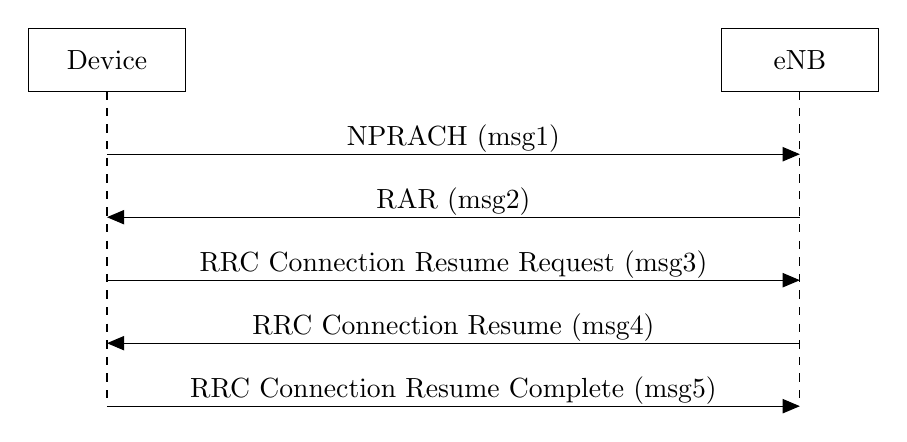
\begin{tikzpicture}[scale = 0.4]

\draw (-13.5,8) rectangle (-8.5,6);
\node at (-11,7) {Device};
\draw [dashed] (-11,6) -- (-11,-4);

\draw (8.5,8) rectangle (13.5,6);
\node at (11,7) {eNB};
\draw [dashed] (11,6) -- (11,-4);

\draw[arrows={-triangle 45}] (-11,4) -- (11,4);
\node at (0,4.5) {NPRACH (msg1)};

\draw[arrows={triangle 45-}] (-11,2) -- (11,2);
\node at (0,2.5) {RAR (msg2)};

\draw[arrows={-triangle 45}] (-11,0) -- (11,0);
\node at (0,0.5) {RRC Connection Resume Request (msg3)};

\draw[arrows={triangle 45-}] (-11,-2) -- (11,-2);
\node at (0,-1.5) {RRC Connection Resume (msg4)};

\draw[arrows={-triangle 45}] (-11,-4) -- (11,-4);
\node at (0,-3.5) {RRC Connection Resume Complete (msg5)};
\end{tikzpicture}
\caption{Message visualisation of the \gls{RAP} for connection resume \citep{NB-IoT_Book}.}
\label{fig:RAP}
\end{figure}

The NPRACH channel, mention in \autoref{sec:ULphy}, is used for transmitting the msg1. With its 12 subcarriers and the jumping pattern shown on \autoref{fig:NPRACH_structure}, does it have 12 different preambles to select between for msg1.

Another important part to take from the \gls{NRAP} is that the device gets a \gls{Ra-RNTI} based on the preamble it selects for msg1. This identifier is used to decode the rest of the messages. During the attach procedure the device is also given a \gls{P-RNTI} and a \gls{C-RNTI}, which is used for decoding radio and paging transmission later on \citep{whitepaper}. If a control plane data transmission is desired it is transmitted during the \gls{NRAP} \citep{primer}.

\subsection{Massiveness}
NB-IoT is designed to handle a massive number of devices (in the orders of thousands). The reason behind this need is that the system has to share its resources with all the devices. There are two points where the massive number of device influence the system: At msg1 in the NRAP, mention in \autoref{sec:RAP} and general usage of the different DL and UL channels.

As described in \autoref{sec:RAP}, are there 12 preambles to use, when wanting to transmit msg1. In the case of multiple devices using the same NPRACH window to transmit msg1, there is a chance that devices chose the same preamble and both transmit it. This duplication of a preamble is first detected at the eNB, when it receives the different msg3, with the same Ra-RNTI, as multiple devices will have the same Ra-RNTI by having used the same preamble. In msg4 do the eNB tell the devices, if it got connected, with no collision at msg1, or that a collision happens at msg1 and gets denied. If a device gets denied, activates it a backoff timer, which value is chosen at random, before transmitting a new preamble. On XXX are shown the success rate for a device not transmitting a preamble chosen by another device. As seen, does the number of devices trying to attach, affect negatively when increasing and with a higher number of devices, does the number of devices trying to attach at the same time increase.

%%Insert beautiful graph

For the general usage of channels in both DL and UL, will a higher number device give more data needed to be transmitted between them and the eNB. With the higher amount of data needed to be transmitted will the devices need to stay in connected state for a longer time, which will consume more battery power. 

\subsection{Connection Control}
A connected device needs to be able to move to the different device states as seen in \autoref{fig:UE-states}. To do this, different procedures are used. The primary concern here is moving in and out of idle modes. Generally, when connected, a device does not want to give up on its \gls{C-RNTI}, as this makes the attach sequence significantly longer, which is where control plane optimization comes in. The control plane optimization enables the device to save its \gls{AS} when it goes into idle mode. This \gls{AS} is then used again, when the device resumes its connection. 

Another aspect is the idle modes, this is where a device is expected to spend most of its time so the power consumption here needs to be minimal. The two primary idle modes are \gls{eDRX} and \gls{PSM}, however, in both modes, a period of time is spent in normal DRX mode. 


\subsubsection{DRX Mode}
When the device wants to disconnect from the network, it might be required to listen for mobile terminated data. This is done through the paging channel. The DRX cycle consists of a paging opportunity and a DRX opportunity, which can be seen on \autoref{fig:DRX_structure}. 

%\tikzsetnextfilename{DRX_structure}
\begin{figure}[H]
\centering
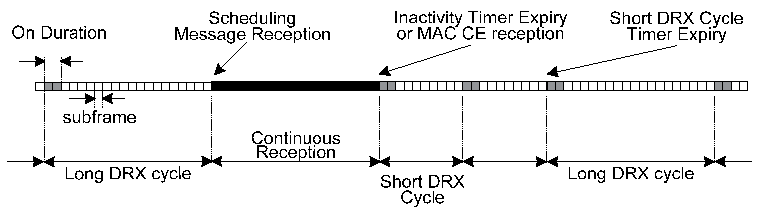
\includegraphics[width=\textwidth]{figures/DRX_structure.pdf}
\caption{The structure of \gls{DRX} idle mode \citep{book_LTE_for_UMTS2}.}
\label{fig:DRX_structure}
\end{figure}

As seen on \autoref{fig:DRX_structure} several parameters define the DRX structure, the different parameters use and typical values can be found in \autoref{tab:DRX_parameters}

\begin{table}[H]
\centering
\begin{tabular}{|c|p{6cm}|p{4cm}|} \hline
\textbf{Parameter} & \textbf{Definition} & \textbf{Typical value} \\ \hline 
On duration &  The number of subframes that is monitored during the paging opportunity & 1-2 subframes\\ \hline
DRX inactivity timer & the period after a scheduling message where the device should be in continuous reception mode & 25-50 subframes \\ \hline
DRX short cycle timer & the duration of the short DRX cycle & 20-40 subframes \\ \hline
Retransmission timer & the period after a \gls{HARQ} round trip time in which the device needs to monitor the control channel & 20  subframes \\ \hline
Long DRX cycle & the duration of the long DRX cycle & 1024 subframes \\ \hline
\end{tabular}
\caption{The different parameters and their typical value when defining the DRX structure \citep{book_LTE_for_UMTS}.}
\label{tab:DRX_parameters}
\end{table}

It should be noted that these typical values are based on the DRX of LTE. In NB-IoT it is uncertain if the short cycle would be used at all and the long cycle might be as long as 10240 subframes. It is also important to note that contrary to LTE, NB-IoT supports repetition of the NPDCCH channel which directly influences the paging messages. \citep{NB-IoT_Book}


\subsubsection{eDRX Mode}
The eDRX idle mode is an extension of the DRX idle mode. It is designed to accommodate a medium length transmission interval. The build-up consist of a long DRX opportunity followed by a normal DRX period often referred to as \gls{PTW}. During the long DRX opportunity only the necessary timers and \gls{PLL}'s, to keep synchronize with the network is powered, as there is no need to listen for incoming data. This cycle can be seen on \autoref{fig:eDRX_structure}.

\tikzsetnextfilename{eDRX_structure}
\begin{figure}[H]
\centering
\resizebox{\textwidth}{!}{
\begin{tikzpicture}

\draw[dashed] (-10,1.5) -- (-1,1.5);
\draw[dashed] (1,1.5) -- (10,1.5);


\draw[dashed] (-10,0) -- (-1,0) node (v4) {};
\draw[dashed] (1,0) node (v5) {} -- (10,0) node (v8) {};
\draw (0,1.5) -- (-0.5,1) -- (0,0.5) -- (-0.5,0);
\draw (0.5,1.5) -- (0,1) -- (0.5,0.5) -- (0,0);
\node at (-10,1.5) {};
\node[anchor=east] at (-10,1.5) {RX:};
\node[anchor=east] (v1) at (-10,0) {Sleep:};
\draw (v1) -- (-9,0) -- (-9,1.5) -- (-8.5,1.5) -- (-8.5,0) node (v2) {};
\draw (v2) -- (-7.5,0) -- (-7.5,1.5) -- (-7,1.5) -- (-7,0) node (v3) {};
\draw (v3) -- (-6,0) -- (-6,1.5) -- (-5.5,1.5) -- (-5.5,0) -- (v4);
\draw (v5) -- (6,0) -- (6,1.5) -- (6.5,1.5) -- (6.5,0) node (v6) {};
\draw (v6) -- (7.5,0) -- (7.5,1.5) -- (8,1.5) -- (8,0) node (v7) {};
\draw (v7) -- (9,0) -- (9,1.5) -- (9.5,1.5) -- (9.5,0) -- (v8);

\draw[arrows={triangle 45- triangle 45}] (-9,-0.5) -- (-7.5,-0.5);
\draw[arrows={triangle 45- triangle 45}] (-9,-1.5) -- (-5.5,-1.5) ;
\draw[arrows={triangle 45- triangle 45}] (-9,-2.5) -- (6,-2.5);
\node at (-8.25,-1) {DRX cycle};
\node at (-7.25,-2) {PTW};
\node at (-1.5,-3) {eDRX cycle};
\end{tikzpicture}}
\caption{The structure of the \gls{eDRX} cycle \citep{NB-IoT_Book}.}
\label{fig:eDRX_structure}
\end{figure}

Two parameters helps define this cycle the eDRX cycle duration, $T_{eDRX}$, and \gls{PTW} duration, $T_{PTW}$. Supported values for these parameters can be seen in \autoref{tab:eDRX_parameters}.

\begin{table}[H]
\centering
\begin{tabular}{|c|p{8cm}|} \hline
\textbf{Parameter} & \textbf{Values in seconds} \\ \hline 
$T_{PTW}$ & 2.56, 5.12, 7.68, 10.24, 12.8, 15.36, 17.92, 20.48, 23.04, 25.6, 28.16, 30.72, 33.28, 35.84, 38.40 and 40.96\\ \hline
$T_{eDRX}$ & 20.48, 40.96, 81.92, 163.84, 327.68, 655.36, 1310.72, 2621.44, 5242.88 and 10485.76 \\ \hline
\end{tabular}
\caption{The different parameters and their typical value when defining the DRX structure \citep{book_LTE_for_UMTS}.}
\label{tab:eDRX_parameters}
\end{table}

\subsubsection{PSM}
The PSM is designed to support long transmission intervals. A DRX period starts the PSM, followed by the PSM state. While in the PSM state, the device is only required to maintain its real-time clock and nothing else. This means that, whenever the device wants to reconnect to the network, it first needs to synchronize itself again. A timer is set when the device enters PSM, this timer defines when the device needs to wake up and perform a \gls{TAU}. This is to keep track of if the device has changed location since it last connected to the network. After a TAU the device enters a DRX period again to enable mobile terminated data transmission. The structure of a PSM cycle can be seen in \autoref{fig:PSM_structure}.

\tikzsetnextfilename{PSM_structure}
\begin{figure}[H]
\centering
\resizebox{\textwidth}{!}{
\begin{tikzpicture}

\draw[dashed] (-10,3) -- (-1,3);
\draw[dashed] (1,3) -- (10,3);

\draw[dashed] (-10,1.5) -- (-1,1.5);
\draw[dashed] (1,1.5) -- (10,1.5);

\draw[dashed] (-10,0) -- (-1,0) node (v4) {};
\draw[dashed] (1,0) node (v5) {} -- (10,0) node (v8) {};

\draw (-0.0157,2.2353) -- (-0.5157,1.7353) -- (-0.0157,1.2353) -- (-0.5157,0.7353);
\draw (0.4843,2.2353) -- (-0.0157,1.7353) -- (0.4843,1.2353) -- (-0.0157,0.7353);

\node[anchor=east] at (-10,3) {TX:};
\node[anchor=east] at (-10,1.5) {RX:};
\node[anchor=east] (v1) at (-10,0) {Sleep:};

\draw (v1) -- (-9,0) -- (-9,3) -- (-7.5,3) -- (-7.5,0) node (v2) {};
\draw (v2) -- (-6.5,0) -- (-6.5,1.5) -- (-6,1.5) -- (-6,0) node (v3) {};
\draw (v3) -- (-5,0) -- (-5,1.5) -- (-4.5,1.5) -- (-4.5,0) -- (v4);
\draw (v5) -- (5,0) -- (5,3) -- (6.5,3) -- (6.5,0) node (v6) {};
\draw (v6) -- (7.5,0) -- (7.5,1.5) -- (8,1.5) -- (8,0) node (v7) {};
\draw (v7) -- (9,0) -- (9,1.5) -- (9.5,1.5) -- (9.5,0) -- (v8);

\draw[arrows={triangle 45- triangle 45}] (-9,-0.5) -- (-7.5,-0.5);
\draw[arrows={triangle 45- triangle 45}] (-7.5,-0.5) -- (-4.5,-0.5) ;
\draw[arrows={triangle 45- triangle 45}] (-4.5,-0.5) -- (5,-0.5);
\node at (-8.25,-1) {TAU};
\node at (-6,-1) {DRX};
\node at (0.25,-1) {PSM};
\end{tikzpicture}}
\caption{The structure of the \gls{PSM} cycle.}
\label{fig:PSM_structure}
\end{figure}

The values for the DRX period and the PSM period is a bit more loosely defined with the possibility of a PSM cycle to take more than a year \citep{NB-IoT_Book}.




